\section{Concurrency: Invariants and Ghost State}
\label{sec:invar-ghost-state}

%% Invariant rules
\newcommand{\invtypingrule}
{\infer{
    \vctx \proves \wtt{\prop}{\Prop} \and
    \vctx \proves \wtt{\iname}{\textlog{InvName}}
  }{
    \vctx \proves \wtt{\knowInv{\iname}{\prop}}{\Prop}
}}
\newcommand{\htmaskweakenrule}[1][]
{\rulegen[#1]{Ht-mask-weaken}
  {S \proves \hoare{P}{e}{v.Q}[\mask_1] \and \mask_1 \subseteq \mask_2}
  {S \proves \hoare{P}{e}{v.Q}[\mask_2]}}
\newcommand{\invpersrule}[1][]
{\rulegen[#1]{Inv-persistent}
{ }
{\knowInv{\iota}{P} \proves \persistently \knowInv{\iota}{P}}}
\newcommand{\htinvallocrule}[1][]
{\rulegen[#1]{Ht-inv-alloc}
{\mathcal{E}\ \infinite \and S \land \Exists \iota \in \mathcal{E}.\knowInv{\iota}{P} \proves \hoare{Q}{e}{v.R}[\mathcal{E}]}
{S \proves \hoare{\later P \ast Q}{e}{v.R}[\mathcal{E}]}}
\newcommand{\htinvopenrule}[1][]
{\rulegen[#1]{Ht-inv-open}
{e \text{ is an atomic expression} \and S \land\knowInv{\iota}{P} \proves \hoare{\later P \ast Q}{e}{v.\later P \ast R}[\mathcal{E}]}
                       {S \land \knowInv{\iota}{P} \proves \hoare{Q}{e}{v.R}[\mathcal{E} \uplus \{\iota\}]}
}
\newcommand{\htframeatomicrule}[1][]
{\rulegen[#1]{Ht-frame-atomic}
  {e \text{ is an atomic expression} \and S \proves \hoare{P}{e}{v.Q}}
  {S \proves \hoare{P \ast \later R}{e}{v.Q \ast R}}}
\newcommand{\htlaterfalserule}[1][]
{\rulegen[#1]{Ht-later-false}
        { e \text{ is an atomic expression} }
        { \hoare{\later(\FALSE)}{e}{v.Q}}}

%% Ghost state rules
\newcommand{\coretypingrule}
{\infer
  {\Gamma \proves \wtt{a}{\Ml_i} \and \mcore{a}_i \text{ defined }}
  {\Gamma \proves \wtt{\mcore{a}_i}{\Ml_i}}}
\newcommand{\validtypingrule}
{\infer
  {\Gamma \proves \wtt{a}{\Ml_i}}
  {\Gamma \proves \wtt{a \in \Vl_i}{\Prop}}}
\newcommand{\owntypingrule}
{\infer
  {\gamma \in \textlog{GhostName} \and \Gamma \proves \wtt{a}{\Ml_i}}
  {\Gamma \proves \wtt{\ownGhost{\gamma}{a : \Ml_i}}{\Prop} }}

%% Update modality rules
\newcommand{\updtypingrule}
{\infer
  {\Gamma \proves \wtt{P}{\Prop}}
  {\Gamma \proves \wtt{\pvs P}{\Prop}}}
\newcommand{\updmonorule}[1][]
{\rulegen[#1]{upd-mono}
  {P \proves Q}
  {\pvs P \proves \pvs Q}}
\newcommand{\updintrorule}[1][]
{\rulegen[#1]{upd-intro}{ }
  {P \proves \pvs P}}
\newcommand{\updidemprule}[1][]
{\rulegen[#1]{upd-idemp}
  { }
  {\pvs \pvs P \proves \pvs P}}
\newcommand{\updframerule}[1][]
{\rulegen[#1]{upd-frame}
  { }
  {P \ast \pvs Q \proves \pvs (P \ast Q)}}


\newcommand{\ownoprule}[1][]
{\rulegen[#1]{Own-op}
  { }
  {\ownGhost{\gamma}{a : \Ml_i} \ast \ownGhost{\gamma}{b : \Ml_i} \provesIff \ownGhost{\gamma}{a \cdot b : \Ml_i}}}
\newcommand{\ownvalidrule}[1][]
{\rulegen[#1]{Own-valid}
  { }
  {\ownGhost{\gamma}{a : \Ml_i} \proves a \in \Vl_i}}
\newcommand{\perscorerule}[1][]
{\rulegen[#1]{Persistently-core}
  {\Gamma \proves \wtt{a}{\Ml_i} \and \mcore{a}_i \text{ defined } }
  {\ownGhost{\gamma}{a : \Ml_i} \proves \persistently \ownGhost{\gamma}{\mcore{a}_i : \Ml_i}}}

\newcommand{\fpurule}[1][]
  {\rulegen[#1]{frame-preserving-update}
    {}{a \mupd B \iff \forall x \in \Ml, a \cdot x \in \Vl \implies \exists b \in B, b \cdot x \in \Vl.}}

\newcommand{\ghostallocrule}[1][]
{\rulegen[#1]{Ghost-alloc}
  {a \in \Vl}
  {\TRUE \proves \pvs \Exists \gamma . \ownGhost{\gamma}{a}}}
\newcommand{\ghostupdaterule}[1][]
{\rulegen[#1]{Ghost-update}
  {a \mupd b}
  { \ownGhost{\gamma}{a} \proves \pvs \ownGhost{\gamma}{b}}}
\newcommand{\htcsqvsrule}[1][]{\htcsqgen[-vs#1]{-vs}{\vs}{}}

%% Derived rules for the update modality
\newcommand{\updseprule}[1][]
{\rulegen[#1]{upd-sep}{P_1 \proves \pvs Q_1 \and P_2 \proves \pvs Q_2}
  {P_1 \ast P_2 \proves \pvs (Q_1 \ast Q_2)}}
\newcommand{\updbindrule}[1][]
{\rulegen[#1]{upd-bind}{P_2 \proves \pvs Q \and P_1 \ast Q \proves \pvs R} {P_1 \ast P_2 \proves \pvs R}}

%% Derived rules for invariants
\newcommand{\htinvallocpostrule}[1][]
{\rulegen[#1]
    {Ht-inv-alloc-post}
    {\mathcal{E}\ \infinite \and S \proves \hoare{P_2}{e}{v.Q}[\mathcal{E}]}
    {S \proves \hoare{\left(\later P_1\right) \ast P_2}{e}{v.Q \land \Exists \iota \in \mathcal{E}.\knowInv{\iota}{P_1}}[\mathcal{E}]}}

In this section we finally extend the logic to support reasoning about concurrent programs.
Two crucial ingredients in achieving this are \emph{invariants} and \emph{ghost state}.
Invariants are used to allow different threads to access the same resources, but in a controlled way, and ghost state is used to keep track of additional information, e.g., relationships between different program variables, needed to verify the program.
Although ghost state is already useful in a sequential setting, it becomes much more powerful and expressive in connection with invariants.

First we introduce the parallel composition construct $\langkw{par}$ with the help of which we will motivate and introduce invariants and ghost state.
Later on we will provide a rule for the \langkw{fork} primitive and derive the rule for the \langkw{par} construct from it.
This derivation however requires more advanced concepts so we postpone it until the next section.
The main reason we use $\langkw{par}$ instead of $\langkw{fork}$ in this section is that it is easier to use in the small motivating examples, since it is a higher-level construct.
\subsection{The par construct}
\label{sec:par-construct}

Using the $\langkw{fork}$ primitive we can implement a ``par'' construct which takes two expressions $e_1$ and $e_2$, runs them in parallel, waits until both finish, and then returns a pair of values to which $e_1$ and $e_2$ evaluated.
First we have the auxiliary methods spawn and join.
We use syntactic sugar $\None$ for $\Inj{1} \TT$ and $\Some x$ for $\Inj{2} x$.

The method $\langkw{spawn}$ takes a function and runs it in another thread, but it also allocates a reference cell.
This cell will hold the result of running the given function.
The method $\langkw{join}$ waits until the value at the given location is $\Some x$ for some value $x$, \ie{} until the flag is set.

\begin{align*}
  \langkw{spawn} &:= \lambda f . \Let c = \Ref(\None) in
                   \langkw{fork}\left(c \gets \Some(f\,())\right); c\\
  \langkw{join} &:= \Rec{f} c = \MatchML{\deref c}with{\Some x}=>{x}|{\None}=> f(c) end{}
\end{align*}

Using these terms we can implement \langkw{par} as follows.
\begin{align*}
  \langkw{par} := \lambda f_1 f_2 . &\Let h = \langkw{spawn} f_1 in\\
                                    &\Let v_2 = f_2\, () in\\
                                    &\Let v_1 = \langkw{join}(h) in\\
                                    &(v_1,v_2)
\end{align*}
Finally, we define new infix notation for the par construct. It
wraps the given expressions into thunks:
\begin{align*}
  e_1 \parcomp e_2 := \langkw{par} (\lambda \_ . e_1) (\lambda \_ . e_2)
\end{align*}
%
In words the functions do the following.  We spawn a new thread and
run the function $f_1$ there.  In the current thread we execute $f_2$
and then wait until $f_1$ finishes (the call to $\langkw{join}$).  The
notation $e_1 \parcomp e_2$ is then a wrapper around $\text{par}$.  We
need to make thunks out of expressions because our language is
call-by-value.  If we were to pass expression $e_1$ and $e_2$ directly
to par, then they would be evaluated in the current thread
\emph{before} being passed to spawn, hence defeating the purpose of
$\text{par}$.

The $\parcomp$ construct satisfies the following specification which we derive in Section~\ref{sec:parcomp-from-fork} from the primitive $\Fork{}$ specification.
\begin{mathpar}
  \inferH{Ht-par}
  {S \proves \hoare{P_1}{e_1}{v.Q_1} \and S \proves \hoare{P_2}{e_2}{v.Q_2}}
  {S \proves \hoare{P_1 \ast P_2}{e_1 \parcomp e_2}{v.\Exists v_1 v_2.v = (v_1,v_2) \ast Q_1[v_1/v] \ast Q_2[v_2/v]}}
\end{mathpar}
The rule states that we can run $e_1$ and $e_2$ in parallel if they 
have \emph{disjoint} footprints and that in this case
we can verify the two components separately. 
Thus this rule is sometimes also referred to as the \emph{disjoint
  concurrency rule}. 

With the concepts introduced so far we can verify simple examples of
concurrent programs.  Namely those where threads do not communicate.
We hasten to point out that there are many important examples of such
programs.  For instance, list sorting algorithms such as quick sort and
merge sort, where the recursive calls operate on disjoint lists of
elements. 

\begin{exercise}
  Prove the following specification.
  \begin{align*}
    \hoare{\ell_1 \pointsto n \ast \ell_2 \pointsto m}{(e_1 \parcomp e_2) ; \deref \ell_1 + \deref \ell_2}{v.v=n + m + 2}
  \end{align*}
  where, for $i \in \{1,2\}$, $e_i$ is the program $\ell_i \gets \deref \ell_i + 1$.
\end{exercise}

However the \ruleref{Ht-par} rule does not suffice
to verify any concurrent programs which modify a shared location.
For instance, we cannot use it to prove
\begin{equation}
  \label{eq:proving-parallel-increments-dont-decrease}
  \hoare{\ell \pointsto n}{(e \parcomp e) ; \deref \ell}{v.v \geq n}
\end{equation}
where $e$ is the program $\ell \gets \deref\ell + 1$.
The problem here is that we cannot split 
the $\ell \pointsto n$ predicate to give to the two subcomputations.

Note that we cannot hope to prove
\begin{align*}
  \hoare{\ell \pointsto n}{(e \parcomp e) ; \deref \ell}{v.v = n + 2}
\end{align*}
since the command $\ell \gets \deref\ell + 1$ is not atomic:
both threads could first read the value stored at $\ell$, 
which is $n$, and then write back the value $n + 1$.

The best we can hope to prove is
\begin{align}
  \label{eq:precise-spec-of-parallel-increment}
  \hoare{\ell \pointsto n}{(e \parcomp e) ; \deref \ell}{v.v = n + 1 \lor v = n + 2}
\end{align}
However this specification is considerably harder to prove than
\eqref{eq:proving-parallel-increments-dont-decrease}. To avoid having
to introduce too many concepts at once, we first focus on describing the
necessary concepts for proving
\eqref{eq:proving-parallel-increments-dont-decrease}.
We return to proving the specification~\eqref{eq:precise-spec-of-parallel-increment} in
Example~\ref{ex:precise-spec-of-parallel-increment} after we introduce the necessary concepts.

What we need is the ability to \emph{share} the predicate $\ell
\pointsto n$ among the two threads running in parallel.
\emph{Invariants} enable such sharing: they are persistent resources,
thus duplicable, and hence sharable among several threads.


\subsection{Invariants}
\label{sec:invariants}

To introduce invariants we need to add a type of invariant names
$\textlog{InvName}$ to the logic.  Invariants are associated with
names and names are used to ensure that we do not open an invariant
more than once.  We explain why this is needed later on.

We add a new term $\knowInv{\iname}{\prop}$ to the logic, which
should be read as invariant $P$ \emph{named} $\iota$, or \emph{associated with the name} $\iota$.

The typing rule for the new construct is as follows.
\begin{align*}
\invtypingrule
\end{align*}
That is, we can make an invariant out of any proposition and any name.
Notice in particular that we can form \emph{nested invariants}, \eg{} terms of the form
$\knowInv{\iname'}{\knowInv{\iname}{P}}$.

The rules for invariants are listed in
Figure~\ref{fig:invariant-rules} on page
\pageref{fig:invariant-rules}.  As mentioned above we need to make
sure that we do not open the same invariant more than once (see
Example~\ref{example:opening-an-invariant-twice} for an example of
what goes wrong if we allow opening an invariant twice).  For this
reason we need to annotate Hoare triples with an infinite set of
invariant names $\El$.  This set identifies the invariants we are
allowed to use; see the rule \ruleref{Ht-inv-open}.  If there is no
annotation on the Hoare triple then $\El = \textlog{InvName}$, the set
of all invariant names.  With this convention all the previous rules
are still valid.

With the addition of invariant names to Hoare triples there is a need
to relate Hoare triples with different sets of invariant names.  We 
just have one rule for that:
\begin{mathpar}
  \htmaskweakenrule
\end{mathpar}
This weakening rule allows us to add more invariant names.
Intuitively it is sound, because if we are \emph{allowed} to use more
invariants then surely we can prove more specifications.

We now explain the rules for invariants.

\paragraph{Invariants are persistent}
The essential property of invariants is that they can be shared by different threads.
The precise way to state this property in Iris is that invariants are persistent (the rule \ruleref{Inv-persistent}).

\paragraph{Allocating invariants}
The invariant allocation rule
\begin{mathpar}
  \htinvallocrule[-inline]
\end{mathpar}
has the following interpretation.  To verify a program $e$, which will
typically contain either $\langkw{fork}$ or parallel composition
$\parcomp$, we want to share the resources described by $P$ between
different threads.  To this end we give away the resources to an
invariant, \ie{} we lose the resources $P$, but we obtain an invariant
$\knowInv{\iota}{P}$ for \emph{some} $\iota$.  We can only specify
that $\iota$ comes from some infinite set of names, but no more.  The
ability to choose $\mathcal{E}$ is needed when we wish to use multiple
invariants.  We want different invariants to be named differently so
that we can open multiple invariants at the same time; see the
explanation of the \ruleref{Ht-inv-open} rule below.

Invariants are persistent, so giving away resources to invariants is
not without cost.  The cost is that invariants can only be used in a
restricted way, namely by the invariant opening rule.

\paragraph{Footprint reading of Hoare triples}
With the introduction of invariants, the ``minimal footprint'' reading
of Hoare triples mentioned in Section~\ref{sec:basic-separation-logic}
must be refined.  Now the resources needed to run the program $e$ can
either be in the precondition $P$ of the triple $\hoare{P}{e}{v.Q}$ or
they can be governed by one or more invariants.  Thus we will often
prove triples of the form $\hoare{\TRUE}{e}{v.Q}$, for some $Q$, where
$e$ accesses shared state governed by an invariant.
See Example~\ref{example:parallel-increments-same-program}, in
particular the proof of the
triple~\eqref{eq:parallel-increments-dont-decrease-allocated-inv} on
page~\pageref{eq:parallel-increments-dont-decrease-allocated-inv}.

Graphically, we can depict the situation as follows.
\begin{center}
  \begin{invdrawing}
\node[
  rectangle split,
  rectangle split horizontal=true,
  rectangle split ignore empty parts=false,
  rectangle split empty part width=15pt,
  rectangle split empty part height=20pt,
  rectangle split parts=10,
  rectangle split part fill={c1,c2,white,c2,c3,c3,white,c1,c1,none},
  line width=1pt,
  draw,
] (heap)
{%
\nodepart[nn]{one}%
\nodepart[nn]{two}%
\nodepart[nn]{three}{$\cdots$}
\nodepart[nn]{four}%
\nodepart[nn]{five}%
\nodepart[nn]{six}%M
\nodepart[nn]{seven}{$\cdots$}%
\nodepart[nn]{eight}%
\nodepart[nn]{nine}%
\nodepart[nn]{ten}{$\cdots$}%
};

\draw [braceover,color=c1] (heap.north west) -- node[above=20pt](I1){} (heap.one split north);
\draw [braceover,color=c1] (heap.seven split north) -- node[above=20pt](I2){} (heap.nine split north);
\draw [braceunder,color=c2] (heap.one split south) -- node[below=20pt](P11){} (heap.two split south);
\draw [braceunder,color=c2] (heap.three split south) -- node[below=20pt](P12){} (heap.four split south);
\draw [braceunder,color=c3] (heap.four split south) -- node[below=20pt](P2){} (heap.six split south);


\draw node[below,thick,minimum width = 40pt,fill=c2](P1node) at ($ (heap.two split south)!0.5!(heap.three split south) - (0,3)$) {$P_1$};
\draw node[below,thick,minimum width = 40pt,fill=c3](P2node) at ($ (heap.four split south)!0.5!(heap.six split south) - (0,3)$) {$P_2$};
\draw node[above,thick,minimum width = 40pt,fill=c1](I1node) at ($ (heap.north west)!0.5!(heap.one split north) + (0,3)$) {$I_1$};
\draw node[above,thick,minimum width = 40pt,fill=c1](I2node) at ($ (heap.seven split north)!0.5!(heap.nine split north) + (0,3)$) {$I_2$};

\draw[line width=2pt,white] (heap.north east) -- (heap.south east);

\draw[thick,color=c2] ($ (P11.center) + (0, 0.44) $) to [bend right=20] (P1node);
\draw[thick,color=c2] ($ (P12.center) + (0, 0.44) $) to [bend left=20] (P1node);
\draw[thick,color=c1] ($ (I2.center) - (0, 0.44)$ ) to [] (I2node);
\draw[thick,color=c1] ($ (I1.center) - (0,0.44) $) to [] (I1node);
\draw[thick,color=c3] ($ (P2.center) + (0, 0.44)$ ) to (P2node);

\end{invdrawing}
\end{center}
The heap (and other resources) is split between local state owned by the two threads (resources $P_1$ owned by the first thread, and resources $P_2$ owned by the second thread) and some shared state owned by invariants (in this case $I_1$ and $I_2$).
Individual threads can access the state owned by invariants and temporarily transfer it to their local state, using the invariant opening rule we will see below.
Thus if, for instance, the first thread opens invariant $I_2$, we can depict the state as follows.
\begin{center}
\begin{invdrawing}
\node[
  rectangle split,
  rectangle split horizontal=true,
  rectangle split ignore empty parts=false,
  rectangle split empty part width=15pt,
  rectangle split empty part height=20pt,
  rectangle split parts=10,
  rectangle split part fill={c1,c2,white,c2,c3,c3,white,c2,c2,white},
  line width=1pt,
  draw,
] (heap)
{%
\nodepart[nn]{one}%
\nodepart[nn]{two}%
\nodepart[nn]{three}{$\cdots$}%
\nodepart[nn]{four}%
\nodepart[nn]{five}%
\nodepart[nn]{six}%M
\nodepart[nn]{seven}{$\cdots$}%
\nodepart[nn]{eight}%
\nodepart[nn]{nine}%
\nodepart[nn]{ten}{$\cdots$}%
};

\draw [braceover,dotted,color=c1] (heap.seven split north) -- node[above=20pt](I2dotted){} (heap.nine split north);
\draw [braceover,color=c1] (heap.north west) -- node[above=20pt](I1){} (heap.one split north);
\draw [braceunder,color=c2] (heap.seven split south) -- node[below=20pt](I2){} (heap.nine split south);
\draw [braceunder,color=c2] (heap.one split south) -- node[below=20pt](P11){} (heap.two split south);
\draw [braceunder,color=c2] (heap.three split south) -- node[below=20pt](P12){} (heap.four split south);
\draw [braceunder,color=c3] (heap.four split south) -- node[below=20pt](P2){} (heap.six split south);

\draw node[below,thick,minimum width = 40pt,fill=c2](P1node) at ($ (heap.two split south)!0.5!(heap.three split south) - (0,3)$) {$P_1$};
\draw node[below,thick,minimum width = 40pt,fill=c3](P2node) at ($ (heap.four split south)!0.5!(heap.six split south) - (0,3)$) {$P_2$};
\draw node[above,thick,minimum width = 40pt,fill=c1](I1node) at ($ (heap.north west)!0.5!(heap.one split north) + (0,3)$) {$I_1$};
\draw node[above,draw=c1,thick,dotted,minimum width = 40pt](I2node) at ($ (heap.seven split north)!0.5!(heap.nine split north) + (0,3)$) {$I_2$};

\draw[line width=2pt,white] (heap.north east) -- (heap.south east);

\draw[thick,color=c2] ($ (P11.center) + (0, 0.44) $) to [bend right=20] (P1node);
\draw[thick,color=c2] ($ (P12.center) + (0, 0.44) $) to [bend left=20] (P1node);
\draw[thick,color=c2] ($ (I2.center) + (-0.005, 0.4)$ ) to [bend left=15] (P1node);
% \draw[thick] (I2.south) to [] (I2node);
\draw[thick,color=c1] ($ (I1.center) - (0,0.44) $) to [] (I1node);
\draw[thick,color=c3] ($ (P2.center) + (0, 0.44)$ ) to (P2node);

\draw[thick, dotted,color=c1] ($ (I2dotted.center) - (0, 0.44)$ ) to [] (I2node);
\end{invdrawing}
\end{center}
The resources owned by the invariant are temporarily transferred to the local state of the first thread.
This is the essence of the invariant opening rule.

\paragraph{Using invariants}
The invariant opening rule
\begin{mathpar}
  \htinvopenrule[-inline]
\end{mathpar}
is the only way to get access to the resources governed by an invariant.
The rule states that if we know an invariant $\knowInv{\iota}{P}$ exists, we can \emph{temporarily}, for one atomic step, get access to the resources.
This rule is the reason we need to annotate the Hoare triples with sets of invariant names $\mathcal{E}$.
This set contains names of those invariants which we are allowed to open.
We refer to $\mathcal{E}$ as a \emph{mask}.
In particular, we cannot open the same invariant twice (see Example~\ref{example:opening-an-invariant-twice} for an example of what goes wrong if we allow opening an invariant twice).

Note that the reader might perhaps be puzzled as to why we need the set of invariant names when we could perhaps just have the rule
\begin{align*}
    \infer
    {e \text{ is an atomic expression} \and S \proves \hoare{\later P \ast Q}{e}{v.\later P \ast R}}
    {S \land \knowInv{\iota}{P} \proves \hoare{Q}{e}{v.R}}
\end{align*}
removing the knowledge about the invariant once we open it.
The reason is that this would not prevent opening invariants in a nested way because the invariant assertion $\knowInv{\iota}{P}$ is persistent.
For this reason from the rule just mentioned we can easily derive
\begin{align*}
    \infer
    {e \text{ is an atomic expression} \and S \land \knowInv{\iota}{P} \proves \hoare{\later P \ast Q}{e}{v.\later P \ast R}}
    {S \land \knowInv{\iota}{P} \proves \hoare{Q}{e}{v.R}}
\end{align*}
which would lead to a contradiction as shown in Example~\ref{example:opening-an-invariant-twice}.

The restriction of the term $e$ to be an \emph{atomic} expression is also essential; see Example~\ref{example:restriction-on-atomic-expr-necessary}.
An expression $e$ is \emph{atomic} if it steps to a value in a single execution step.

\paragraph*{Existing Hoare triple rules}
The existing rules for Hoare triples, \eg{} those in Figure~\ref{fig:hoare-triple-rules-sequential}, are all still valid with arbitrary masks, but the premises and conclusions of the rules must be annotated with the same mask.
For example, the rule \ruleref{Ht-beta} becomes 
\newcommand{\htbetamask}[1][]{\htbetagen[-mask#1]{ }{\mask}}
\begin{mathpar}
  \htbetamask
\end{mathpar}
for an arbitrary invariant mask $\mask$.

The rules in Figure~\ref{fig:invariant-rules} will be considerably
\emph{generalised} and \emph{simplified} later, but for that we
need concepts we have not yet introduced.

Before proceeding with an example we need one more rule, namely a
stronger frame rule, which is only applicable in certain cases.  The
rule is needed because opening invariants only gives access to the
resources \emph{later}.  This is essential.  The logic would be
inconsistent otherwise, though proof of this fact is not yet within
our reach.\footnote{The precise statement and proof of this property can be found in~\cite{iris-ground-up}, although it uses concepts we have not yet introduced here.}

The stronger frame rule is the following 
\begin{mathpar}
  \htframeatomicrule
\end{mathpar}
%
This rule is useful because typically an invariant will contain
something akin to $\ell \pointsto v$, plus some additional facts about
$v$, and the expression $e$ will be either reading from or writing to the
location $\ell$.  This rule, together with the invariant opening rule,
allows us to get the facts about $v$ \emph{now} (note that there is no
$\later$ on $R$ in the postcondition) after reading the
value.

\begin{exercise}[Later False]
  \label{exercise:later-false-hoare-triples}
  We will often use an invariant to tell us that some cases are impossible.
  For instance an invariant will often encode a transition system, e.g., encoding a communication protocol, and different threads will hold tokens which will be used to guarantee that the transition system can only be in certain states, meaning, for instance, that a certain message has not yet been sent.
  Thus we will have some resources \emph{now} that are incompatible with those held by the invariant.
  But the invariant gives us those resources, and hence the inconsistency, \emph{later}.
  Using \ruleref{Ht-frame-atomic} show the following triples.
  \begin{mathpar}
    { \hoare{\later(\FALSE)}{\ell\gets v}{v. Q} }\and
    { \hoare{\later(\FALSE)}{!\ell}{v. Q} }\and
    { \hoare{\later(\FALSE)}{\Ref(v)}{v. Q} }\and
    { \hoare{\later(\FALSE)}{\CAS(\ell,v_1,v_2)}{v. Q} }    
  \end{mathpar}  
  and use them to derive the following rule.
  \begin{mathpar}
    \htlaterfalserule
  \end{mathpar}
  Hint: use \ruleref{Ht-csq} with the fact that $\FALSE$ entails anything and $\later$ is monotone (the rule \ruleref{Later-Mono}).
\end{exercise}


\begin{figure}[htbp]
  \centering
  \begin{mathpar}
    \invpersrule
    \and
    \htinvallocrule
    \and
    \htinvopenrule
  \end{mathpar}
  \caption{Rules for invariants.}
  \label{fig:invariant-rules}
\end{figure}

\begin{example}[Opening an invariant twice leads to an inconsistency]
  \label{example:opening-an-invariant-twice}
  This example demonstrates a problem with opening an invariant more than once.
  Suppose the invariant opening rule \ruleref{Ht-inv-open} did not remove the name $\iota$ from the possible set of invariants to open, \ie{} suppose the rule was instead
  \begin{mathpar}
    \infer
    {e \text{ is an atomic expression} \and S \land\knowInv{\iota}{P} \proves \hoare{\later P \ast Q}{e}{v.\later P \ast R}[\mathcal{E}\uplus \{\iota\}]}
    {S \land \knowInv{\iota}{P} \proves \hoare{Q}{e}{v.R}[\mathcal{E} \uplus \{\iota\}]}
  \end{mathpar}
  Then we can derive the following nonsensical triple.
  \begin{align*}
    \hoare{\ell \pointsto 0}{\deref \ell}{v.v = 3}.
  \end{align*}
  Indeed, using the invariant allocation rule \ruleref{Ht-inv-alloc}
  we just need to prove
  \begin{align*}
    \Exists \iota \in \textlog{InvName}.\knowInv{\iota}{\ell \pointsto 0} \proves
    \hoare{\TRUE}{\deref\ell}{v.v=3}.
  \end{align*}
  Opening the invariant once we have to show
  \begin{align*}
    \knowInv{\iota}{\ell \pointsto 0} \proves \hoare{\later(\ell \pointsto 0)}{\deref \ell}{v.v=3 \land \later(\ell \pointsto 0)}.
  \end{align*}
  And opening again we need to show
  \begin{align*}
    \knowInv{\iota}{\ell \pointsto 0} \proves \hoare{\later (\ell \pointsto 0 \ast \ell \pointsto 0)}{\deref \ell}{v.v=3 \land \later(\ell \pointsto 0 \ast \ell \pointsto 0)}.
  \end{align*}
  Since $\ell \pointsto 0 \ast \ell\pointsto 0$ is equivalent to $\FALSE$ we can use \ruleref{Ht-later-false} to prove the triple.

  Hence opening the same invariant twice cannot be allowed.
\end{example}

\begin{example}
  \label{example:parallel-increments-same-program}
  We now have sufficient rules to prove specification
  \eqref{eq:proving-parallel-increments-dont-decrease} from page
  \pageref{eq:proving-parallel-increments-dont-decrease}.
  \begin{align*}
    \hoare{\ell \pointsto n}{(e \parcomp e) ; \deref \ell}{v.v \geq n}.
  \end{align*}
  We start off by allocating an invariant.  One might first guess that
  the invariant is $\ell \pointsto n$.  However this does not work
  since the value at location $\ell$ does in fact change, so is not
  \emph{invariant}.  Technically, we can see that, to use the invariant
  opening rule, we need to reestablish the invariant (the $\later P$ in
  the post-condition).

  Instead, we use the weaker predicate
  $I = \Exists m.m \geq n \land \ell \pointsto m$, which is an
  invariant.  To show
  \eqref{eq:proving-parallel-increments-dont-decrease} we first
  allocate the invariant $I$ using \ruleref{Ht-inv-alloc}.  This we
  can do by the rule of consequence \ruleref{Ht-csq} since
  $\ell \pointsto n$ implies $I$, and so also $\later I$.

  Thus we have to prove
  \begin{align}
    \label{eq:parallel-increments-dont-decrease-allocated-inv}
    \knowInv{\iota}{I} \proves \hoare{\TRUE}{(e \parcomp e) ; \deref \ell}{v.v \geq n}
  \end{align}
  for some $\iota$.

  Using the derived sequencing rule \ruleref{Ht-seq} we need to show the following two triples
  \begin{align*}
    \knowInv{\iota}{I} &\proves \hoare{\TRUE}{(e \parcomp e)}{\_.\TRUE}.\\
    \knowInv{\iota}{I} &\proves \hoare{\TRUE}{\deref \ell}{v.v\geq n}.
  \end{align*}

  We show the first one; during the proof of that
  we will need to show the second triple as well.
  Using the rule \ruleref{Ht-par}, the proof of the first triple reduces to showing
  \begin{align*}
    \knowInv{\iota}{I} \proves \hoare{\TRUE}{e}{\_.\TRUE}
  \end{align*}
  where, recall,  $e$ is the term $\ell \gets \deref\ell + 1$.
  Note that we cannot open the invariant now since the expression $e$ is not atomic.

  Using the bind rule we first show
  \begin{align*}
    \knowInv{\iota}{I} \proves \hoare{\TRUE}{\deref \ell}{v.v \geq n}.
  \end{align*}
  Note that this is exactly the second premise of the sequencing rule mentioned above.
  To show this triple, we use the invariant opening rule
  \ruleref{Ht-inv-open},
  and thus it remains to show
  \begin{align*}
    \hoare{\later I}{\deref \ell}{v.v \geq n \land \later I}[\textlog{InvName} \setminus \{\iota\}].
  \end{align*}
  
  Using the rule \ruleref{Ht-frame-atomic} together with the rule
  \ruleref{Ht-load} and structural rules we have
  \begin{align*}
    \hoare{\later I}{\deref \ell}{v.v = m \land m \geq n \land \ell \pointsto m}[\textlog{InvName} \setminus \{\iota\}].
  \end{align*}
  From this we easily derive the needed triple.

  To show the second premise of the bind rule we need to show
  \begin{align*}
    \knowInv{\iota}{I} \proves \All m . \hoare{m \geq n}{\ell \gets (m + 1)}{\_.\TRUE}.
  \end{align*}
  To show this we again use the invariant opening rule and \ruleref{Ht-frame-atomic}.
  \begin{exercise}
    Show this claimed specification in detail.
  \end{exercise}
  
  This concludes the proof.
\end{example}

\begin{example}[Restriction to atomic expressions in \ruleref{Ht-inv-open} is necessary.]
  \label{example:restriction-on-atomic-expr-necessary}
  The restriction on atomic expressions in the invariant opening rule is necessary.
  Consider the following program, call it $e$
  \begin{align*}
    (\ell \gets 4 ; \ell \gets 3) \parcomp \deref \ell
  \end{align*}
  and the invariant $I = \ell \pointsto 3$.
  Suppose the rule \ruleref{Ht-inv-open} did not restrict expressions $e$ to be atomic.
  Then we could allocate the invariant $\knowInv{\iota}{I}$ and
  then use the rule \ruleref{Ht-par}.
  Without the atomicity restriction it is easy to show (exercise!)
  \begin{align*}
    \knowInv{\iota}{I} \proves \hoare{\TRUE}{\ell \gets 4; \ell \gets 3}{\_.\TRUE}
  \end{align*}
  and 
  \begin{align*}
    \knowInv{\iota}{I} \proves \hoare{\TRUE}{\deref \ell}{v.v = 3}
  \end{align*}
  Hence, by \ruleref{Ht-par}, we conclude
  \begin{align*}
    \hoare{\ell \pointsto 3}{e}{v.v = ((), 3)}.
  \end{align*}
  However, the pair $((),
  4)$ is also a possible result of executing
  $e$ (the second thread could read $\ell$ just after it was set to
  $4$ by the first thread).  Thus the logic would not be sound with
  respect to the operational behaviour of the programming language.
\end{example}

\subsection{A peek at ghost state}
\label{sec:peek-at-ghost}

The specification \eqref{eq:proving-parallel-increments-dont-decrease}
is weaker than what happens operationally.  The following
specification
\begin{equation}
  \label{eq:proving-parallel-increments-increase-at-least-by-one}
  \hoare{\ell \pointsto n}{(e \parcomp e) ; \deref \ell}{v.v \geq n + 1}
\end{equation}
where $e$ is again the program $\ell \gets \deref\ell + 1$ is sound.
However the logic we have introduced thus far does not allow us to
prove it.  Invariants allow us to make resources available to
different threads, but exactly because they are shared by different
threads, the resources governed by them need to be preserved, \ie{} the
invariant has to be reestablished after each step of execution.  Thus,
for instance, when the invariant is $\ell \pointsto n$ the location
$\ell$ must always point to the value $n$.

We could allow the state to change by using an invariant such as
$\ell \pointsto n \lor \ell \pointsto (n+1)$.  However with the
concepts introduced until now we cannot have an invariant that would
ensure that once $\ell \pointsto (n+1)$ holds, the location $\ell$ will
never point to $n$ again.

One way to express this is using \emph{ghost state}.  In
Iris, ghost state is an additional kind of primitive resource,
analogous to the points-to predicate.  Other names for the same
concept are \emph{auxiliary state}, \emph{logical state}, or \emph{abstract state}, to
contrast it with \emph{concrete state}, which is the concrete program
configuation, \ie{} a heap and threadpool.

Iris supports a uniform treatment of ghost state, but in this
subsection we start out
more concretely, with just enough ghost state to prove specification~\eqref{eq:proving-parallel-increments-increase-at-least-by-one}.

To work with ghost state we extend Iris with a new type 
$\textlog{GhostName}$ of \emph{ghost names}, 
which we typically write as $\gamma$.
Ghost names are to be thought of as analogous to concrete
locations in the heap, but for the abstract state of the program.
Hence ghost names are also sometimes referred to as ghost variables.
There are no special operations on ghost names.  Ghost names can only
be introduced by ghost name allocation, which we explain below.

\newcommand{\stok}{\textsc{S}}
\newcommand{\ftok}{\textsc{F}}

To prove
\eqref{eq:proving-parallel-increments-increase-at-least-by-one} we
need two additional primitive resource propositions, indexed by
$\textlog{GhostName}$: $\ownGhost{\gamma}{\stok}$ and
$\ownGhost{\gamma}{\ftok}$.  These satisfy the following basic
properties:
\begin{mathpar}
  \infer[\ftok-\text{duplicable}]
  { }
  {\ownGhost{\gamma}{\ftok} \proves \ownGhost{\gamma}{\ftok} \ast \ownGhost{\gamma}{\ftok}}
  \and
  \infer[\stok-\stok-\text{incompatible}]
  { }
  {\ownGhost{\gamma}{\stok} \ast \ownGhost{\gamma}{\stok} \proves \FALSE}
  \and
  \infer[\stok-\ftok-\text{incompatible}]
  { }
  {\ownGhost{\gamma}{\stok} \ast \ownGhost{\gamma}{\ftok} \proves \FALSE}
\end{mathpar}
The way to think about these propositions is that
$\ownGhost{\gamma}{\stok}$ is the ``start'' token.  The invariant will
start out in this ``state''.  The proposition
$\ownGhost{\gamma}{\ftok}$ is the ``finished'' token.  Once the
invariant is in this state, it can never go back to the state
$\ownGhost{\gamma}{\stok}$.

Conceptually, the tokens are used to encode the following transition system.
\begin{center}
  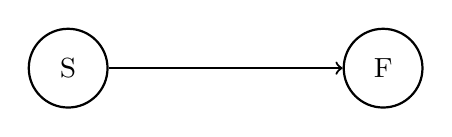
\begin{tikzpicture}[term/.style={circle,draw,minimum size=10mm,inner sep=5pt},auto]
    \node [thick] (s) at (0,0) [term] {$\stok$};
    \node [thick] (f) at (4,0) [term] {$\ftok$};
    \draw [->,thick] (s) to (f);
  \end{tikzpicture}
\end{center}

Additionally, we need rules relating these tokens to Hoare triples:
\begin{mathpar}
  \inferH{Ht-token-alloc}
  {T \in \{\stok, \ftok\} \and
    S \proves \hoare{\Exists \gamma.\ownGhost{\gamma}{T} \ast P}{e}{v.Q}}
  {S \proves \hoare{P}{e}{v.Q}}
  \and
  \inferH{Ht-token-update-pre}
  {S \proves \hoare{\ownGhost{\gamma}{\ftok} \ast P}{e}{v.Q}}
  {S \proves \hoare{\ownGhost{\gamma}{\stok} \ast P}{e}{v.Q}}
  \and
  \inferH{Ht-token-update-post}
  {S \proves \hoare{P}{e}{v.\ownGhost{\gamma}{\stok} \ast Q}}
  {S \proves \hoare{P}{e}{v.\ownGhost{\gamma}{\ftok} \ast Q}}
\end{mathpar}
%
Using these rules, we now
prove \eqref{eq:proving-parallel-increments-increase-at-least-by-one}.
The invariant we pick is the following predicate,
parametrised by $\gamma \in \textlog{GhostName}$.
\begin{align*}
  I(\gamma) = \Exists m. \ell \pointsto m \ast \left(\left(\ownGhost{\gamma}{\stok} \land m \geq n\right) \lor
                                                     \left(\ownGhost{\gamma}{\ftok} \land m \geq (n+1)\right)\right)
\end{align*}
%
The idea is as explained above.  The invariant can be in two
``states''.  It will be allocated in the first state, with the
``start'' token $\stok$, since we know that the current value stored
at $\ell$ is at least $n$.  Then, when a thread increases the value
stored at $\ell$, we
will update the invariant, so that it is in the ``finished'' state.
This pattern of using special ghost state tokens and disjunction to
encode information about the execution of the program in the invariant
is typical, and we shall see more of it later.

\begin{example}
  \label{example:parallel-increment-at-least-1}
So, let us start proving.
We start off by using the rule \ruleref{Ht-token-alloc} plus
\ruleref{Ht-exist}, so we have to prove
\begin{align*}
  \hoare{\ownGhost{\gamma}{\stok} \ast \ell \pointsto n}{(e \parcomp e) ; \deref \ell}{v.v \geq n + 1}.
\end{align*}
We then again use the sequencing rule \ruleref{Ht-seq}, but this time
the intermediate proposition is not $\TRUE$, but
$\ownGhost{\gamma}{\ftok}$, \ie{} we prove the following two triples
\begin{align}
  &\hoare{\ownGhost{\gamma}{\stok} \ast \ell \pointsto n}{e \parcomp e}{v.\ownGhost{\gamma}{\ftok}}\\
  &\hoare{\ownGhost{\gamma}{\ftok}}{\deref \ell}{v.v \geq n+1}.
    \label{eq:parallel-increments-second-triple}
\end{align}
We begin by showing the first triple.  Start by using the invariant
allocation rule \ruleref{Ht-inv-alloc}.  This is allowed by an
application of the rule of consequence \ruleref{Ht-csq} since
$\ownGhost{\gamma}{\stok} \ast \ell \pointsto n$ implies $I(\gamma)$.
Hence we have to prove
\begin{align*}
  \knowInv{\iota}{I(\gamma)} \proves \hoare{\TRUE}{e \parcomp e}{v.\ownGhost{\gamma}{\ftok}}.
\end{align*}
Since $\ownGhost{\gamma}{\ftok} \ast \ownGhost{\gamma}{\ftok}$ implies $\ownGhost{\gamma}{\ftok}$ it suffices (by the rule of consequence) to use the parallel composition rule \ruleref{Ht-par} and prove 
\begin{align*}
  \knowInv{\iota}{I(\gamma)} \proves \hoare{\TRUE}{e}{v.\ownGhost{\gamma}{\ftok}}.
\end{align*}
%
Again, using the bind rule, we first need to prove
\begin{align*}
  \knowInv{\iota}{I(\gamma)} \proves \hoare{\TRUE}{\deref \ell}{v.v \geq n}.
\end{align*}
Exercise!

For the other premise of the bind rule, we now have to show
\begin{align*}
  \knowInv{\iota}{I(\gamma)} \proves \hoare{m \geq n}{\ell \gets (m + 1)}{\_.\ownGhost{\gamma}{\ftok}}.
\end{align*}
To open the invariant we need an atomic expression.
We use the rule \ruleref{Ht-bind-det} to evaluate $m + 1$ to a value using the rule \ruleref{Ht-op}.
We then open the invariant and after using the rule \ruleref{Ht-disj} and other structural rules we need to prove the following two triples
\begin{align*}
  &\knowInv{\iota}{I(\gamma)} \proves \hoare{\later (\ell \pointsto m \ast \ownGhost{\gamma}{\stok} \land m \geq n)}
    {\ell \gets (m + 1)}{\_.\later I(\gamma) \ast \ownGhost{\gamma}{\ftok}}\\
  &\knowInv{\iota}{I(\gamma)} \proves \hoare{\later (\ell \pointsto m \ast \ownGhost{\gamma}{\ftok} \land m \geq (n+1))}
    {\ell \gets (m + 1)}{\_.\later I(\gamma) \ast \ownGhost{\gamma}{\ftok}}
\end{align*}
We only show the first one, and leave the second one as an exercise.
We note however that duplicability of $\ownGhost{\gamma}{\ftok}$ is essential.

Using the rules \ruleref{Ht-frame-atomic} and \ruleref{Ht-store} we derive the following entailment.
\begin{align*}
  &\knowInv{\iota}{I(\gamma)} \proves
    \hoare{\later (\ell \pointsto m \ast \ownGhost{\gamma}{\stok} \land m \geq n)}
    {\ell \gets (m + 1)}{v.v = () \land \ell \pointsto (m + 1) \ast \ownGhost{\gamma}{\stok} \land m \geq n}
\end{align*}
Following up with \ruleref{Ht-token-update-post} we get
\begin{align*}
  &\knowInv{\iota}{I(\gamma)} \proves
    \hoare{\later (\ell \pointsto m \ast \ownGhost{\gamma}{\stok} \land m \geq n)}
    {\ell \gets (m + 1)}{v.v = () \land \ell \pointsto (m + 1) \ast \ownGhost{\gamma}{\ftok} \land m \geq n}
\end{align*}
from which it is easy to derive the wanted triple using \textsc{\ftok-duplicable} to create another copy of $\ownGhost{\gamma}{\ftok}$.
One of the copies is used to reestablish the invariant $I(\gamma)$, and the other remains in the postcondition.

To conclude the proof of this example we now need to show \eqref{eq:parallel-increments-second-triple}
\begin{align*}
  \knowInv{\iota}{I(\gamma)} \proves \hoare{\ownGhost{\gamma}{\ftok}}{\deref \ell}{v.v \geq n + 1}
\end{align*}
%
Using the invariant opening rule \ruleref{Ht-inv-open} together with
structural rules we need to prove
\begin{align*}
  &\knowInv{\iota}{I(\gamma)} \proves \hoare{\ownGhost{\gamma}{\ftok} \ast \later (\ell \pointsto m \ast \ownGhost{\gamma}{\stok} \land m \geq n)}
    {\deref \ell}{v.v \geq (n + 1) \land \later I(\gamma)}\\
  &\knowInv{\iota}{I(\gamma)} \proves
    \hoare{\ownGhost{\gamma}{\ftok} \ast \later (\ell \pointsto m \ast \ownGhost{\gamma}{\ftok} \land m \geq (n + 1))}
    {\deref \ell}{v.v \geq (n + 1) \land \later I(\gamma)}
\end{align*}
By \textsc{\stok-\ftok-incompatible}, the precondition of the first triple is equivalent to $\later\FALSE$, that is, this case is \emph{impossible}, and the triple holds by \ruleref{Ht-later-false}.
We leave the second triple as an exercise.

To recap, the high-level idea of the proof is that the invariant can
be in two ``states''.  It starts off in the state where we know that
the value at $\ell$ is at least $n$ and then, when incrementing, we
transition to a new state, but we also get out a new token, \ie{} we
get $\ownGhost{\gamma}{\ftok}$ in the postcondition.  This token
is then used to decide in which case we are when opening the invariant
again.
\end{example}

\subsection{Ghost state}
\label{sec:ghost-state}

The ghost state used in the previous section was rather \emph{ad hoc}.
If we had to extend the logic with new primitive propositions for each new example, we would need to establish consistency for each such extension.
That is not tenable.
Thus in this section we develop a very general notion of resources.
It is not the most general notion of resources supported by Iris, but the final generalisation is quite technical and postponed until later sections.
Consistency of Iris with respect to this notion of resources will be proved in later sections.
The notion of resources described in this section suffices for the vast majority of program verifications.
However it is insufficient for certain more advanced uses of the logic, such as when Iris is used to reason about refinement, or when building the Iris program logic on top of the base logic.

\newcommand{\valid}{\mathcal{V}}

To define the notion of resources we need to recall some concepts and facts.
\begin{definition}
  A \emph{commutative semigroup} is a set $\Ml$ together with a function
  $(\cdot) : \Ml \times \Ml \to \Ml$, called the \emph{operation} such that
  the operation is associative and commutative.

  A commutative semigroup is called a \emph{commutative monoid} if there exists an 
  element $\eps$ (called the unit) which is the neutral element for the operation $(\cdot)$: for all
    $m \in \Ml$, the property $m \cdot \eps = \eps \cdot m = m$ holds.

  The set $\Ml$ is called the \emph{carrier} of the semigroup (resp.~monoid).
\end{definition}

Every semigroup can be made a preorder by defining the \emph{extension order} $a \mincl b$ as
\begin{align*}
  a \mincl b \iff \exists c, b = a \cdot c.
\end{align*}
In words, $a \mincl b$ if $a$ \emph{is a part of} $b$.
\begin{exercise}
  Show that the relation $\mincl$ is transitive for any semigroup $\Ml$.
  Show that it is reflexive if and only if for every element $a$ there exists an element $b \in \Ml$ such that $a \cdot b = a$.
  Conclude that if $\Ml$ is a commutative monoid then $\mincl$ is reflexive.
\end{exercise}


Certain kinds of commutative semigroups and monoids serve as good abstract models of resources.
Resources can be composed using the operation.
Commutativity and associativity express that the order in which resources are composed does not matter.
The unit of the monoid represents the empty resource, which exists in many instances.

Finally, we also need the ability to express that certain resources cannot be combined together.
This can be achieved in many ways.
The way we choose to do it is to have a subset $\Vl$ of so-called \emph{valid elements}.
Thus, for now, our notion of resources are the resource algebras defined as follows.%
\footnote{In general, resources in Iris can be elements of so-called ``cameras'' which are generalizations of \emph{resource algebras}.
  They add additional \emph{approximation information} to resources which is needed for the most advanced applications, however the vast majority of program verifications needs only the ``discrete cameras'', which is what we call resource algebras in these lecture notes.}
\begin{definition}[Resource algebra]
  \label{def:resource-algebra}
  A \emph{resource algebra} is a commutative semigroup $\Ml$ together with a subset $\Vl \subseteq \Ml$ of elements called \emph{valid}, and a \emph{partial} function $\mcore{\cdot} : \Ml \to \Ml$, called the \emph{core}.

  The set of valid elements is required to have the closure property
  \begin{align*}
    a \cdot b \in \Vl \implies a \in \Vl,
  \end{align*}
  that is, if $x$ is valid then every sub-part of $x$ is also valid.
  
  The core is required to have the following properties.
  \begin{align*}
    \mcore{a} \text{ defined} &\implies \mcore{a}\cdot a = a\\
    \mcore{a} \text{ defined} &\implies \mcore{\mcore{a}} = \mcore{a}\\
    a \mincl b \land \mcore{a} \text{ defined} &\implies \mcore{b} \text{ defined } \land \mcore{a} \mincl \mcore{b}.
  \end{align*}

  A resource algebra is \emph{unital} if $\Ml$ is a commutative monoid with unit $\eps$ and the following properties hold.
  \begin{mathpar}
    \eps \in \Vl \and \mcore{\eps} = \eps.
  \end{mathpar}
  In particular $\mcore{\eps}$ is defined.
\end{definition}
The core of the resource algebra is meant to be a function, which for each element captures the ``duplicable part'' of an element.
Sometimes such a duplicable part does not exist, hence we allow the core to be a partial function; we will see some such examples below.
\begin{exercise}
  Show that for any resource algebra $\Ml$, and any element $a \in \Ml$, the core of $a$, if defined, is duplicable, \ie{} for any $a$, show
  \begin{align*}
    \mcore{a} \text{ defined} \implies \mcore{a} \cdot \mcore{a} = \mcore{a}.
  \end{align*}
\end{exercise}


\begin{exercise}
  \label{exercise:unital-ra-core-total}
  Show that in a unital resource algebra the core is always defined.
  Hint: $\eps \mincl a$ for any element $a$.
\end{exercise}


\begin{example}
  \label{example:unital-resource-algebra-of-heaps}
  A canonical example of a unital resource algebra is the one of heaps.
  More precisely, the carrier of the resource algebra is the set of heaps plus an additional element, call it $\bot$, which is used to define composition of incompatible heaps.
  Composition of heaps is disjoint union, and if the heaps are not disjoint, then their composition is defined to be $\bot$.
  Composing $\bot$ with any other element yields $\bot$.
  The core is the constant function, mapping every element to the empty heap, which is the unit of the resource algebra.
  Every heap is valid, the only non-valid element being $\bot$.
\end{example}

\begin{example}
  \label{example:agreement-resource-algebra}
  We now present an example, which we will use later, and where the core is non-trivial.
  (It is closely related to the \emph{agreement construction}, which we will also use later on.)
  Given a set $X$, the carrier of the resource algebra is the set $X \cup \{\bot\}$, for some element $\bot$ not in $X$.
  The operation $(\cdot)$ is defined by the following rules.
  The non-trivial compositions are only
  \begin{mathpar}
    m \cdot m = m
  \end{mathpar}
  and otherwise (when $m$ and $n$ are distinct) $m \cdot n = \bot$.
  The core can be defined as the identity function, and every element apart from $\bot$ is valid.
  The definition of the core as the identity function is possible since every element of the resource algebra is duplicable.
\end{example}

\begin{example}[Finite subsets of natural numbers]
  \label{example:finite-subset-resource-algebra}
  The carrier of this resource algebra is the set of finite subsets of natural numbers and an additional element $\bot$. The operation is disjoint union, i.e.:
  \begin{align*}
    x \cdot y = 
    \begin{cases}
      x \cup y & \text{ if } x \cap y = \emptyset\\
      \bot & \text{ otherwise }
    \end{cases}
  \end{align*}

The unit of this operation is $\emptyset$. Valid elements are all finite subsets of natural numbers and the core operation maps every valid element to $\emptyset$.
\end{example}

\begin{example}
  \label{example:two-state-transition-system-ra}
  If we take the resource algebra $M$ to have the carrier $\{\stok, \ftok,\bot\}$ with multiplication defined as $\ftok \cdot \ftok = \ftok$ and otherwise $x \cdot y = \bot$ then, with the rules presented above, we can recover the rules \textsc{ftok-duplicable}, \textsc{\stok-\stok-incompatible} and \textsc{\stok-\ftok-incompatible}, which were postulated in the previous section.
  The core of the resource algebra $M$ is always undefined.
\end{example}

\begin{example}[Resource algebra of fractions]
  \label{example:resource-algebra-of-fractions}
  An often used resource algebra is the one of fractions $\QQ_{01}$.
  Its carrier is the set of (strictly) positive rational numbers $q$ with addition as the operation.
  However the valid elements are only those $q$ less than or equal to $1$, \ie{} ${\Vl = \left\{ q \isetsep 0 < q \leq 1 \right\}}$.
  The core is always undefined.
\end{example}

\begin{example}[Exclusive resource algebra]
  \label{ex:exclusive-resource-algebra}
  Given a set $X$ the exclusive resource algebra $\exm(X)$ has as carrier the set $X$ with an additional element $\bot$.
  The operation is defined such that $x \cdot y = \bot$ for all $x$ and $y$.
  The core is the always undefined function, and the valid elements are elements of $X$, \ie{} every element of the resource algebra except the $\bot$.

  Perhaps it does not seem that this resource algebra is very interesting.
  In fact it does appear in verification of certain programs, but it can also be used as a building block of other resource algebras, as shown in the following exercise.
\end{example}

The following examples are generic constructions.
They construct resource algebras combined from a variety of smaller ones.
This makes it easier to build more complex notions of resources needed in verification, since a lot of the infrastructure can be reused.
However it does take some practice to get used to thinking in terms of decomposition of the desired resource algebra in terms of the smaller ones.
We hope the reader will get some intuition for this by working through the example verifications in the rest of these notes.

\begin{example}[Products of resource algebras]
  If $\Ml_1$ and $\Ml_2$ are resource algebras with cores $\mcore{\cdot}_1$ and $\mcore{\cdot}_2$ and sets of valid elements $\Vl_1$ and $\Vl_2$ then we can form the product resource algebra $\Ml_\times$.
  Its carrier is the product $\Ml_1 \times \Ml_2$, and its operation is defined component-wise as
  \begin{align*}
    (a, b) \cdot (a', b') = (a \cdot a', b \cdot b')
  \end{align*}
  and the set of valid elements
  \begin{align*}
    \Vl_\times = \left\{(a, b) \isetsep a \in \Vl_1, b \in \Vl_2\right\}.
  \end{align*}
  The core is similarly defined component-wise as
  \begin{align*}
    \mcore{(a, b)}_\times =
    \begin{cases}
      \left(\mcore{a}_1, \mcore{b}_2\right) & \text{ if } \mcore{a}_1 \text{ and } \mcore{b}_2 \text{ defined}\\
      \text{undefined} & \text{ otherwise }
    \end{cases}
  \end{align*}
  It is easy to see (exercise!) that if both resource algebras are unital then so is the product resource algebra.

  This product example can be extended to a product of arbitrary many resource algebras.
\end{example}

\begin{example}[Finite map resource algebra]
  Let $(\Ml, \Vl, \mcore{\cdot})$ be a resource algebra.
  We can form a new resource algebra $\NN \finparmap \Ml$ whose carrier is the set of partial functions from $\NN$ to $\Ml$ with finite domain, and the operation is defined as
  \begin{align*}
    (f \cdot g)(n) =
    \begin{cases}
      f(n) \cdot g(n) & \text{ if } f(n) \text{ and } g(n) \text{ defined}\\
      f(n) & \text{ if } f(n) \text{ defined and} g(n) \text{ undefined}\\
      g(n) & \text{ if } g(n) \text{ defined and} f(n) \text{ undefined}\\
      \text{ undefined} & \text{ otherwise}
    \end{cases}
  \end{align*}
  The set of valid finite maps is
  \begin{align*}
    \Vl_{\NN \finparmap \Ml} = \left\{f \isetsep \forall n, f(n) \text{ defined} \implies f(n) \in \Vl\right\}
  \end{align*}
  and the core is defined as
  \begin{align*}
    (\mcore{f}_{\NN \finparmap \Ml})(n) =
    \begin{cases}
      \mcore{f(n)} & \text{ if } f(n) \text{ and } \mcore{f(n)} \text{ defined }\\
      \text{ undefined} & \text{ otherwise }
    \end{cases}
  \end{align*}
  Note that $\NN \finparmap \Ml$ is always a \emph{unital} resource algebra, its unit being the always undefined finite partial function.
\end{example}

\begin{exercise}
  Show that when restricted to valid elements, the resource algebra $\NN \finparmap \exm\left(\Val\right)$ is the same as the unital resource algebra of heaps described in Example~\ref{example:unital-resource-algebra-of-heaps}.
  More precisely, show that the valid elements of $\NN \finparmap \exm\left(\Val\right)$ are precisely the heaps, and composition of these is exactly the same as the composition of heaps, if it is a valid element.
\end{exercise}


\begin{example}[Option resource algebra]
  \label{example:option-resource-algebra}
  Given any resource algebra (not necessarily unital) $\Ml$, we define the unital resource algebra $\Ml_?$.
  Its carrier is the set $\Ml$ together with a new element $?$.
  The operation on elements of $\Ml$ is inherited, and we additionally set $? \cdot x = x \cdot ? = x$, \ie{} $?$ is the unit.
  The set of valid elements is that of $\Ml$ and $?$.
  Finally, the core operation is defined as
  \begin{align*}
    \mcore{?}_{\Ml_?} &={} ?\\
    \mcore{x}_{\Ml_?} &=
                \begin{cases}
                  \mcore{x} & \text{ if } \mcore{x} \text{ defined}\\
                  ? & \text{ otherwise}
                \end{cases}
  \end{align*}
\end{example}

\paragraph*{Extending Iris with resource algebras}
With these concepts, we can extend Iris with a general notion of resources, a single unital resource algebra.
Strictly speaking the logic is extended with a family of chosen resource algebras $\Ml_i$, which we leave open, so that new ones can be added when they are needed in the verification of concrete examples.
We add the resource algebras, and its elements, the core function, and the property of the element being valid, as new types and new terms of the logic, together with all the equations for the operations.
In addition to this we also add the notion of ghost names.
These are used to be able to refer to multiple different instances of the same resource algebra element, analogous to how different locations in a heap are used to contain different values.

Thus we extend the logic with the following constructs
\begin{mathpar}
  \coretypingrule
  \and
  \validtypingrule
  \and
  \owntypingrule
\end{mathpar}
The first two are self-explanatory, they internalise the notions of the resource algebra into the logic, \ie{} they allow us to reason about elements of the resource algebras in the logic.
The last rule introduces a new construct, the \emph{ghost ownership assertion} $\ownGhost{\gamma}{a : \Ml_i}$, which we will write as $\ownGhost{\gamma}{a}$ when the resource algebra $\Ml_i$ is clear from the context.
This assertion states that we own an instance of a ghost resource $a$ named $\gamma$.

The rules of the ghost ownership assertion are as follows.
\begin{mathpar}
  \ownoprule
  \and
  \ownvalidrule
\end{mathpar}
And the final rule, which shows why the core is useful, is related to the persistently modality with the following law of the logic.
\begin{mathpar}
  \perscorerule
\end{mathpar}

\paragraph*{Ghost updates}
We now consider how to update the ghost resources.
This ability will be used to evolve the ghost state along with the execution of the program.
When the ghost state changes, it is important that it remains valid -- Iris always maintains the invariant that the ghost state obtained by composing the contributions of all threads is well-defined and valid, \ie{} that all the contributions of all threads are compatible.
We call state changes that maintain this invariant \emph{frame-preserving updates}.

\begin{definition}[Frame preserving update]
  \label{def:frame-preserving-update}
  For any resource algebra $\Ml$ with the set of valid elements $\Vl$ we define a relation, the \emph{frame preserving update} $a \mupd B$, where $a \in \Ml$ and $B \subseteq \Vl$ is a \emph{non-empty} subset of valid elements.
  It states that any element compatible with $a$ is compatible with \emph{some} element in $B$.
  Precisely,
  \begin{mathpar}
    \fpurule
  \end{mathpar}
  If $B$ is the singleton set $\{b\}$, we write $a \mupd b$ for $a \mupd \{b\}$.
\end{definition}
%
To support modification of ghost state in the logic we introduce a new
\emph{update modality} $\pvs P$, with associated frame preserving
updates.  The typing rules and basic axioms of the update modality are
show in Figure~\ref{fig:pvs}.  The intuition is that $\pvs P$ holds
for a resource $r$, if from $r$ we can do a frame-preserving update to
some $r'$ that satisfies $P$. Thus the update modality $\pvs P$
provides a way, inside the logic, to talk about the resources we
\emph{could} own after performing an update to what we \emph{do} own.
With this intuitive reading of $\pvs P$, the laws in
Figure~\ref{fig:pvs} should make sense. For instance, the
\ruleref{upd-frame} axiom holds because if $r$ satisfies
$P \ast \pvs Q$, then $r$ can be split into $r_1$ and $r_2$ with
$r_1$ in $P$ and $r_2$ in $\pvs Q$, and the latter means that $r_2$
can be updated in a frame-preserving way to some $r'_2$ in $Q$, \ie{}
$r_2\mupd r'_2$.  But then also
$r=(r_1 \cdot r_2) \mupd (r_1 \cdot r'_2)$ and hence
$r\in\pvs (P \ast Q)$.

\begin{figure}[htbp]
  \centering
\begin{mathpar}
  \updtypingrule
  \and
  \updmonorule
  \and
  \updintrorule
  \and
  \updidemprule
  \and
  \updframerule
\end{mathpar}
  \caption{Laws for the update modality}
  \label{fig:pvs}
\end{figure}

\begin{exercise}
\label{exercise:basic-properties-of-primitive-view-shift}
  Show the following derived rules.
  \begin{enumerate}
  \item
    \begin{mathpar}
      \infer{P_1 \proves Q_1 \and P_2 \proves \pvs Q_2}
      {P_1 \ast P_2 \proves \pvs (Q_1 \ast Q_2)}
    \end{mathpar}
  \item 
    \begin{mathpar}
      \updseprule
    \end{mathpar}
  \item
    \begin{mathpar}
      \updbindrule
    \end{mathpar}
  \end{enumerate}
\end{exercise}


\begin{remark}
  Note that the rule \ruleref{upd-bind} is a kind of bind or let rule.
  Indeed, it may be instructive to compare the rule \ruleref{upd-bind}
  with the typing rule for a let construct in an ML-like language
\begin{mathpar}
  \infer
  {\Gamma \proves e_1 : \tau \and \Gamma, x : \tau \proves e_2 : \sigma}
  {\Gamma \proves \Let x = e_1 in e_2 : \sigma}
\end{mathpar}
The difference is that because of the use of separating conjunction we
need to separate the resources needed to prove $\pvs Q$ from those
needed to prove the $\pvs R$.  Thus we cannot use $P_2$ anymore when
proving $\pvs R$.
Instead \ruleref{upd-bind} very closely corresponds to the let rule in a language with an affine or linear type system.

The following exercise shows that if a more standard let-like rule is
added to the logic then the update modality would become significantly weaker.
\end{remark}

\begin{exercise}
  Show that if the rule
  \begin{mathpar}
    \infer{P \proves \pvs Q \and P \ast Q \proves \pvs R} {P \proves \pvs R}
  \end{mathpar}
  is added to the logic then the following is derivable for any $R$.
  \begin{mathpar}
    \infer
    {P \ast P \proves \FALSE}
    {P \proves \pvs R}
  \end{mathpar}
  In particular $P \proves \pvs \FALSE$ for $P$ such that $P \ast P \proves \FALSE$.
\end{exercise}


The update modality allows us to allocate 
and update ghost resources, as explained by the following rules.
\begin{mathpar}
  \ghostallocrule
  \and
  \ghostupdaterule
\end{mathpar}

Finally, we connect the update modality with Hoare triples.  The idea
is that ghost state is abstract state used to keep track of auxiliary
facts during proofs.  So we should be able to update the
ghost state in pre- and postconditions of Hoare triples,
since whether or not the program is safe to run, and its return value, only depends on the physical state.

A uniform way to do this is to generalise the consequence rule \ruleref{Ht-csq}.
We first define the \emph{view shift} $P \vs Q$ as
\begin{align*}
  P \vs Q = \persistently(P \implies \pvs Q)
\end{align*}
The generalized rule of consequence is then 
\begin{mathpar}
  \htcsqvsrule
\end{mathpar}
\begin{exercise}
  Derive the previous rule of consequence from the one just introduced.
\end{exercise}


\begin{exercise}
  \label{exercise:basic-properties-of-view-shift}
  Derive the following.
  
  \begin{itemize}
  \item
    \begin{align*}
      \infer
      {a \in \Vl}
      {P \proves \pvs \left(\left(\Exists \gamma.\ownGhost{\gamma}{a}\right) \ast P\right)}
    \end{align*}
  \item 
    \begin{displaymath}
      \infer
      {a \in \Vl}
      {\proves P \vs \left(\Exists \gamma.\ownGhost{\gamma}{a}\right) \ast P} \qedhere
    \end{displaymath}
  \end{itemize}
\end{exercise}


In particular, we have $\TRUE \vs \Exists \gamma.\ownGhost{\gamma}{a}$, for all valid $a$, and if $a \mupd b$ then $\ownGhost{\gamma}{a} \vs \ownGhost{\gamma}{b}$.
\begin{exercise}
  Derive the rest of the rules for start and finish tokens used in the previous section for the resource algebra from Example~\ref{example:two-state-transition-system-ra}.
  That is, show the rules \ruleref{Ht-token-update-post}, \ruleref{Ht-token-update-pre}, and \ruleref{Ht-token-alloc}.
\end{exercise}


\begin{exercise}[Allocating invariants in the post-condition]
  \label{exercise:allocating-invariants-postcondition}
  It will often be the case that we need to allocate an invariant in the post-condition, using the following derivable rule.
  \begin{mathpar}
    \htinvallocpostrule
  \end{mathpar}
  Derive the rule using \ruleref{Ht-inv-alloc}, the fact that invariants are persistent and the generalised rule of consequence introduced above.
\end{exercise}


\begin{example}
  \label{ex:precise-spec-of-parallel-increment}
  In this example we show how to use slightly more complex reasoning using resource algebras to show the specification~\eqref{eq:precise-spec-of-parallel-increment} (page~\pageref{eq:precise-spec-of-parallel-increment}) from the parallel increment example.
  We are going to use two resource algebras: the one of fractions defined in Example~\ref{example:resource-algebra-of-fractions} together with the resource algebra encoding the transition system with states $\stok$ and $\ftok$ defined in Example~\ref{example:two-state-transition-system-ra} and demonstrated in Example~\ref{example:parallel-increment-at-least-1}.
  
  The proof proceeds similarly to the proof in Example~\ref{example:parallel-increment-at-least-1}, but with a different invariant.
  The invariant we are going to use is
  \begin{align*}
    I(\gamma_1, \gamma_2, n) =\ &\ell \pointsto n \ast \ownGhost{\gamma_1}{\stok} \lor\\
                                &\ell \pointsto (n+1) \ast \ownGhost{\gamma_1}{\ftok} \ast \ownGhost{\gamma_2}{\frac{1}{2}}\lor\\
                                &\ell \pointsto (n+2) \ast \ownGhost{\gamma_1}{\ftok} \ast \ownGhost{\gamma_2}{1}
  \end{align*}
  That is, we are in essence encoding a three state transition system.
  The tokens $\ftok$ and $\stok$ are used to distinguish the initial state from the rest of the states, and the fractions $\frac{1}{2}$ and $1$ can be thought of as the price needed to get from the initial state to the current state.
  We can depict this in the following way
  \begin{center}
    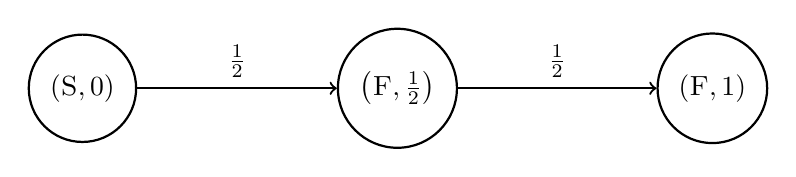
\begin{tikzpicture}[term/.style={circle,draw,minimum size=10mm,inner sep=5pt},auto]
      \node [thick] (s) at (0,0) [term] {$(\stok, 0)$};
      \node [thick] (f1) at (4,0) [term] {$\left(\ftok, \frac{1}{2}\right)$};
      \node [thick] (f2) at (8,0) [term] {$(\ftok, 1)$};
      \draw [->,thick] (s) to node {$\frac{1}{2}$} (f1);
      \draw [->,thick] (f1) to node {$\frac{1}{2}$} (f2);
    \end{tikzpicture}
  \end{center}
  The resources on the transitions can also be viewed as coming from the environment.
  To make a transition from one state to another the environment will have to give up ownership of $\ownGhost{\gamma_2}{\frac{1}{2}}$ and transfer it to the invariant.

  With this invariant let us proceed to the proof of the specification
  \begin{align*}
    \hoare{\ell \pointsto n}{(e \parcomp e) ; \deref \ell}{v.v = n + 1 \lor v = n + 2}.
  \end{align*}
  We start off by allocating two pieces of ghost state.
  We allocate $\ownGhost{\gamma_1}{\stok}$ and $\ownGhost{\gamma_2}{1}$ for some $\gamma_1$ and $\gamma_2$ using the rule \ruleref{Ghost-alloc} and the generalized rule of consequence.
  Hence we have to show
  \begin{align*}
      \hoare{\ownGhost{\gamma_1}{\stok} \ast \ownGhost{\gamma_2}{1} \ast \ell \pointsto n}{(e \parcomp e) ; \deref \ell}{v.v = n + 1 \lor v = n + 2}.
  \end{align*}
  Using the invariant allocation rule we allocate the invariant by transferring
  \begin{align*}
    \ownGhost{\gamma_1}{\stok} \ast \ell \pointsto n
  \end{align*}
  into the invariant, which then means we have to show
  \begin{align*}
    \knowInv{\iota}{I(\gamma_1,\gamma_2,n)} \proves \hoare{\ownGhost{\gamma_2}{1}}{(e \parcomp e) ; \deref \ell}{v.v = n + 1 \lor v = n + 2}
  \end{align*}
  for some $\iota$.
  Using the rule \ruleref{Ht-seq} we now verify the two parts, showing the following two triples
  \begin{align*}
    \knowInv{\iota}{I(\gamma_1,\gamma_2,n)} &\proves \hoare{\ownGhost{\gamma_2}{1}}{(e \parcomp e)}{\_.\ownGhost{\gamma_1}{\ftok}}\\
    \knowInv{\iota}{I(\gamma_1,\gamma_2,n)} &\proves \hoare{\ownGhost{\gamma_1}{\ftok}}{\deref \ell}{v.v = n + 1 \lor v = n + 2}.\\
  \end{align*}
  The proof of the second triple is completely analogous to the one in Example~\ref{example:parallel-increment-at-least-1}, so we omit it here.
  To show the first triple we first use the rule \ruleref{Own-op} to get
  \begin{align*}
    \ownGhost{\gamma_2}{1} \iff \ownGhost{\gamma_2}{\frac{1}{2}} \ast \ownGhost{\gamma_2}{\frac{1}{2}}
  \end{align*}
  and 
  \begin{align*}
    \ownGhost{\gamma_1}{\ftok} \iff \ownGhost{\gamma_1}{\ftok} \ast \ownGhost{\gamma_1}{\ftok}
  \end{align*}
  and hence the first triple is equivalent to
  \begin{align*}
    \knowInv{\iota}{I(\gamma_1,\gamma_2,n)} &\proves \hoare{\ownGhost{\gamma_2}{\frac{1}{2}} \ast \ownGhost{\gamma_2}{\frac{1}{2}}}{(e \parcomp e)}{\_.\ownGhost{\gamma_1}{\ftok} \ast \ownGhost{\gamma_1}{\ftok}}
  \end{align*}
  which means we can use the parallel composition rule \ruleref{Ht-par}, and we have to show
  \begin{align*}
    \knowInv{\iota}{I(\gamma_1,\gamma_2,n)} &\proves \hoare{\ownGhost{\gamma_2}{\frac{1}{2}}}{e}{\_.\ownGhost{\gamma_1}{\ftok}}.
  \end{align*}
  Recall that $e$ is the program $\ell \gets \deref \ell + 1$.
  Using the \ruleref{Ht-bind} rule we show the following two entailments.
  \begin{align}
    \label{eq:parallel-increment-reading-spec}
    \knowInv{\iota}{I(\gamma_1,\gamma_2,n)} &\proves \hoare{\ownGhost{\gamma_2}{\frac{1}{2}}}{\deref \ell}{v.\left(v = n \lor v = (n+1) \ast \ownGhost{\gamma_1}{\ftok}\right) \ast \ownGhost{\gamma_2}{\frac{1}{2}}}\\
    \label{eq:parallel-increment-writing-spec}
    \knowInv{\iota}{I(\gamma_1,\gamma_2,n)} &\proves \All v .\hoare{\left(v = n \lor v = (n+1) \ast \ownGhost{\gamma_1}{\ftok}\right)\ast \ownGhost{\gamma_2}{\frac{1}{2}}}{\ell \gets v + 1}{\_.\ownGhost{\gamma_1}{\ftok}}
  \end{align}
  Note the $\ownGhost{\gamma_1}{\ftok}$ token we chose to add in the postcondition for the case of reading $n+1$. As in Example~\ref{example:parallel-increment-at-least-1}, this is essential to show the second triple: with $\ownGhost{\gamma_1}{\ftok}$ being duplicable, this allows us to \emph{remember} that the invariant is not in the initial state anymore.
  Then, when storing, we can exclude the impossible case where we store $n+2$ (and thus must have read $n+1$) while the invariant is still in the initial state $\ownGhost{\gamma_1}{\stok}$ (in which case we would not be able to reestablish the invariant, as we only have one $\ownGhost{\gamma_2}{\frac{1}{2}}$ fraction).
  As in this case we will have ownership of both the S and the F token (which are incompatible), we will be able to reach a contradiction.

  We first show \eqref{eq:parallel-increment-reading-spec} and start by opening the invariant $I(\gamma_1,\gamma_2,n)$.
  We thus get
  \begin{align*}
    \later\left(\ell \pointsto n \ast \ownGhost{\gamma_1}{\stok} \lor \ell \pointsto (n+1) \ast \ownGhost{\gamma_1}{\ftok} \ast \ownGhost{\gamma_2}{\frac{1}{2}}\lor                               \ell \pointsto (n+2) \ast \ownGhost{\gamma_1}{\ftok} \ast \ownGhost{\gamma_2}{1}\right) \ast \ownGhost{\gamma_2}{\frac{1}{2}}
  \end{align*}
  in the precondition which, using the distributivity laws of the logic, together with \ruleref{Own-op} simplifies to
  \begin{align*}
    &\later\left(\ell \pointsto n \ast \ownGhost{\gamma_1}{\stok}\right) \ast \ownGhost{\gamma_2}{\frac{1}{2}} \lor\\
    &\later \left(\ell \pointsto (n+1) \ast \ownGhost{\gamma_1}{\ftok} \ast \ownGhost{\gamma_2}{\frac{1}{2}}\right) \ast \ownGhost{\gamma_2}{\frac{1}{2}} \lor\\
    &\later\left(\ell \pointsto (n+2) \ast \ownGhost{\gamma_1}{\ftok} \ast \ownGhost{\gamma_2}{\frac{3}{2}}\right)
  \end{align*}
  The last disjunct is equivalent to $\later \FALSE$ by \ruleref{Own-valid} and the fact that the only valid fractions are those which are not greater than $1$.
  Using the disjunction rule \ruleref{Ht-disj} we have to show further three triples, all with postcondition 
  \begin{align*}
    \left(v = n \lor v = (n+1) \ast \ownGhost{\gamma_1}{\ftok}\right) \ast \ownGhost{\gamma_2}{\frac{1}{2}} \ast \later I(\gamma_1,\gamma_2,n)
  \end{align*}
  and with three preconditions corresponding to the three disjuncts above.
  The last is the easiest one and follows directly from \ruleref{Ht-later-false}.
  The first two we leave as exercises, since they are direct applications of rules we have seen many times.
  \begin{exercise}
    Show the following two triples.
    \begin{align*}
      &\hoare{\later\left(\ell \pointsto n \ast \ownGhost{\gamma_1}{\stok}\right) \ast \ownGhost{\gamma_2}{\frac{1}{2}}}{\deref \ell}{v.\left(v = n \lor v = (n+1) \ast \ownGhost{\gamma_1}{\ftok}\right) \ast \ownGhost{\gamma_2}{\frac{1}{2}} \ast \later I(\gamma_1,\gamma_2,n)}\\
      &\hoare{\later \left(\ell \pointsto (n+1) \ast \ownGhost{\gamma_1}{\ftok} \ast \ownGhost{\gamma_2}{\frac{1}{2}}\right) \ast \ownGhost{\gamma_2}{\frac{1}{2}}}{\deref \ell}{v.\left(v = n \lor v = (n+1) \ast \ownGhost{\gamma_1}{\ftok}\right) \ast \ownGhost{\gamma_2}{\frac{1}{2}} \ast \later I(\gamma_1,\gamma_2,n)}
    \end{align*}
  \end{exercise}
  
  
  Let us now turn to showing the specification \eqref{eq:parallel-increment-writing-spec}.
  Using the $\forall$ introduction rule, distributivity of $\ast$ over $\lor$, and \ruleref{Ht-disj} this means showing two specifications. 
  \begin{align}
    \label{eq:parallel-increment:read-n}
    \knowInv{\iota}{I(\gamma_1,\gamma_2,n)} &\proves \hoare{v = n \ast \ownGhost{\gamma_2}{\frac{1}{2}}}{\ell \gets v + 1}{\_.\ownGhost{\gamma_1}{\ftok}}\\
    \label{eq:parallel-increment:read-n-one}
    \knowInv{\iota}{I(\gamma_1,\gamma_2,n)} &\proves \hoare{v = (n+1) \ast \ownGhost{\gamma_1}{\ftok} \ast \ownGhost{\gamma_2}{\frac{1}{2}}}{\ell \gets v + 1}{\_.\ownGhost{\gamma_1}{\ftok}}
  \end{align}
  We show the first and leave the second as an exercise.
  Using \ruleref{Ht-persistently} and ordinary equational reasoning the first triple is equivalent to
  \begin{align*}
    \knowInv{\iota}{I(\gamma_1,\gamma_2,n)} &\proves \hoare{\ownGhost{\gamma_2}{\frac{1}{2}}}{\ell \gets n + 1}{\_.\ownGhost{\gamma_1}{\ftok}}
  \end{align*}
  To be completely precise we first need to use the bind rule to compute $n + 1$ to a value, but this is completely straighforward, so let us just assume we have done it.
  We then open the invariant and after simplifying we have
  \begin{align*}
    \later\left(\ell \pointsto n \ast \ownGhost{\gamma_1}{\stok} \ast \ownGhost{\gamma_2}{\frac{1}{2}}\right) \lor
    \later \left(\ell \pointsto (n+1) \ast \ownGhost{\gamma_1}{\ftok} \ast \ownGhost{\gamma_2}{1}\right) \lor
    \later\left(\ell \pointsto (n+2) \ast \ownGhost{\gamma_1}{\ftok} \ast \ownGhost{\gamma_2}{\frac{3}{2}}\right)
  \end{align*}
  in the precondition.
  As before, the last disjunct is equivalent to $\later\FALSE$ and the corresponding triple follows from \ruleref{Ht-later-false}.
  Using \ruleref{Ht-disj} we thus need to prove the following two specifications.
  \begin{align}
    \label{eq:parallel-increment:write:we-have-read-n}
    &\hoare{\later\left(\ell \pointsto n \ast \ownGhost{\gamma_1}{\stok} \ast \ownGhost{\gamma_2}{\frac{1}{2}}\right)}{\ell \gets n+1}{\_.\ownGhost{\gamma_1}{\ftok} \ast \later I(\gamma_1,\gamma_2,n)}\\
    \label{eq:parallel-increment:write:we-have-read-n-one}
    &\hoare{\later \left(\ell \pointsto (n+1) \ast \ownGhost{\gamma_1}{\ftok} \ast \ownGhost{\gamma_2}{1}\right)}{\ell \gets n+1}{\_.\ownGhost{\gamma_1}{\ftok} \ast \later I(\gamma_1,\gamma_2,n)}
  \end{align}
  We show the first and leave the second as an exercise.
  We proceed by forward reasoning and start by using \ruleref{Ht-load} and \ruleref{Ht-frame-atomic} to get
  \begin{align}
    \label{eq:1:needs-consequence}
    \hoare{\later\left(\ell \pointsto n \ast \ownGhost{\gamma_1}{\stok} \ast \ownGhost{\gamma_2}{\frac{1}{2}}\right)}{\ell \gets n+1}
    {\ell \pointsto n+1 \ast \ownGhost{\gamma_1}{\stok} \ast \ownGhost{\gamma_2}{\frac{1}{2}}}
  \end{align}
  We then use the fact that $\stok \mupd \ftok$ together with the rule \ruleref{Ghost-update} and \ruleref{upd-frame} to get
  \begin{align*}
    \left(\ell \pointsto n+1 \ast \ownGhost{\gamma_1}{\stok} \ast \ownGhost{\gamma_2}{\frac{1}{2}}\right) \vs \left(\ell \pointsto n+1 \ast \ownGhost{\gamma_1}{\ftok} \ast \ownGhost{\gamma_2}{\frac{1}{2}}\right)
  \end{align*}
  Moreover $\ftok = \ftok \cdot \ftok$ and thus \ruleref{Own-op} gives us $\ownGhost{\gamma_1}{\ftok} \vs \left(\ownGhost{\gamma_1}{\ftok} \ast \ownGhost{\gamma_1}{\ftok}\right)$ and thus together we have
  \begin{align*}
    \left(\ell \pointsto n+1 \ast \ownGhost{\gamma_1}{\stok} \ast \ownGhost{\gamma_2}{\frac{1}{2}}\right) \vs
    \left(\ell \pointsto n+1 \ast \ownGhost{\gamma_1}{\ftok} \ast \ownGhost{\gamma_1}{\ftok} \ast \ownGhost{\gamma_2}{\frac{1}{2}}\right).
  \end{align*}
  Clearly $\ell \pointsto n+1 \ast \ownGhost{\gamma_1}{\ftok} \ast \ownGhost{\gamma_2}{\frac{1}{2}} \vs \later I(\gamma_1,\gamma_2,n)$ and thus we have
  \begin{align*}
    \left(\ell \pointsto n+1 \ast \ownGhost{\gamma_1}{\stok} \ast \ownGhost{\gamma_2}{\frac{1}{2}}\right) \vs
    \left(\ownGhost{\gamma_1}{\ftok} \ast \later I(\gamma_1,\gamma_2,n)\right)
  \end{align*}
  and thus finally, by the (generalized) rule of consequence, we get \eqref{eq:parallel-increment:write:we-have-read-n} from \eqref{eq:1:needs-consequence}, as needed.
  
  \begin{exercise}
    Following similar reasoning illustrated above show specifications~\eqref{eq:parallel-increment:write:we-have-read-n-one} and~\eqref{eq:parallel-increment:read-n-one}.
  \end{exercise}
  

  The proof is somewhat complex, and perhaps the key new point, compared to previous examples (in particular Example~\ref{example:parallel-increment-at-least-1}), is lost to the reader.
  The key new way of reasoning in this example is the use of the fraction $\frac{1}{2}$ and how we transferred it from the ownership of a thread to the ownership of the invariant.
  Technically this can be seen from the fact that if when reading $\deref \ell$ the invariant is in state $\ell \pointsto n \ast \ownGhost{\gamma_1}{\stok}$, then after writing it is in state $\ell \pointsto (n+1) \ast \ownGhost{\gamma_1}{\ftok} \ast \color{red} \ownGhost{\gamma_2}{\frac{1}{2}}$.
  Analogously, if the invariant is in state
  $\ell \pointsto (n+1) \ast \ownGhost{\gamma_1}{\ftok} \ast \color{red} \ownGhost{\gamma_2}{\frac{1}{2}}$ when reading, then after writing it is in state $\ell \pointsto (n+2) \ast \ownGhost{\gamma_1}{\ftok} \ast \color{red} \ownGhost{\gamma_2}{1}$.
  Finally, we have used the fact that the threads own $\ownGhost{\gamma_2}{\frac{1}{2}}$ at the beginning, to discount the possibility that
  we have read the value $n+2$ before writing, \ie{} that the invariant was in state $\ell \pointsto (n+2) \ast \ownGhost{\gamma_1}{\ftok} \ast \color{red} \ownGhost{\gamma_2}{1}$.
\end{example}
\begin{exercise}
  For the same program $e$ as in the preceding example, define an invariant which would allow you to prove the following specification
  \begin{align*}
    \hoare{\ell \pointsto n}{\left((e \parcomp e) \parcomp e\right) ; \deref \ell}{v. v = n+1 \lor v = n+2 \lor v = n+3}.
  \end{align*}
\end{exercise}


\begin{example}
  \label{example:parallel-add}
  This example is a generalization of the parallel increment example~\ref{ex:precise-spec-of-parallel-increment}.
  Instead of for a fixed number of threads, we will prove a specification for any number of threads adding to a location.
  We also generalize it to the addition of any number instead of just $1$ for each thread.
  This is slightly more interesting, because the possible result values in the location are not just $n+1, n+2, \ldots, n+k$, but any combination of the numbers the threads are adding.
  As we will see, this does not allow us to use the same reasoning as in the previous example.
  Instead, we present another way of combining state-tracking resource algebras (multiple S-F instances), which at the same time represents an alternative way of proving the specification of Example~\ref{ex:precise-spec-of-parallel-increment}, without using the fractional resource algebra.

  Another new aspect of this example is that we show a specification for an inductively constructed program, namely a program consisting of any number of nested threads. As we will see in the proof, induction on the list of threads while having an invariant about those threads is not trivial.

  The program and specification for $k$ threads with numbers $a_1, \ldots, a_k$ to add is the following:
  \newcommand{\paralleladdprog}[1][k]{\left(e_1 \parcomp\;(e_2 \parcomp\;\cdots\;(e_{#1-1} \parcomp e_{#1})\cdots\right))}
  \begin{align}
    \label{eq:parallel-add-spec}
    \hoare{\ell \pointsto n}
    {\paralleladdprog \; ; \; \deref \ell}
    {v. \exists A \subseteq \{1,\dots,k\}\,,\; A \neq \emptyset \;\land\; v = n + \textstyle\sum_{i \in A}{a_i} }
  \end{align}
  where $e_i \;=\; \ell \gets \deref \ell + a_i$.

  The proof is structured as the one in Example~\ref{ex:precise-spec-of-parallel-increment}:
  We will have an invariant that governs the location $\ell$ and which can be in different states, logically representing which threads have contributed.
  One might think that we could proceed with fractions similarly to the example with two threads where instead of a fraction $\frac{1}{2}$, each thread would get a fraction corresponding to its contribution, \ie{} $\frac{a_j}{\sum_{i=1,\dots,k} a_i}$ for thread $j$, and the fractions collected in the invariant would represent the amount added to the location.
  However, this will not work out, as we will not be able to distinguish between the addition of an $a_i$ and two times the addition of $\frac{a_i}{2}$, for instance.
  This would allow to represent sums that in reality are not possible.

  Luckily, it turns out that the problem is much simpler and we do not even need fractions.
  What we actually want to track is whether a thread has contributed or not, to discount the possibility of a thread's number being contributed twice.
  This can be achieved with the two-state transition system with states S and F from Example~\ref{example:two-state-transition-system-ra} which we also have used in the previous proofs of parallel increment.
  We will simply use $k$ instances of this resource algebra, one for each thread.
  We use the ghost names $\overline\gamma = \gamma_1, \dots, \gamma_k$ to distinguish them.
  Additionally we will -- as before -- use the same transition system to encode the global state of execution, namely whether we are in the starting state S or a final state F.
  This instance is represented by the ghost name $\gamma$.
  With this idea, our invariant looks as follows:
  \begin{align*}
    I(\gamma,\overline\gamma, n) =\ \ell \pointsto n \ast \ownGhost{\gamma}{\stok} \;\lor\;
                                               \exists A \subseteq \{1,\dots,k\}\,,\; A \neq \emptyset \;\land\; \ell \pointsto n + \textstyle\sum_{i \in A}{a_i} \;\ast\; \Sep_{i \in A}\; \ownGhost{\gamma_i}{\ftok} \ast \ownGhost\gamma\ftok
  \end{align*}
  The invariant can be in two states. The first state, represented by the token $\ownGhost{\gamma}{\stok}$, is the same as in the example with just two threads: the value at the location is unchanged, as no thread has written to the location yet.
  The second state, represented by the token $\ownGhost{\gamma}{\ftok}$, represents all possible final states of the program, \ie{} where all threads have executed and thus the contribution of at least one thread has to have been added to $\ell$.
  For each thread whose number is included in the sum, we additionally have the thread-specific final state token $\ownGhost{\gamma_i}{\ftok}$.
  This allows us to exclude the impossible case where a thread's number is already part of the sum when it makes its contribution.

  Let us now show how we can prove specification \eqref{eq:parallel-add-spec} using this invariant.
  We start by allocating ghost state: the global $\ownGhost{\gamma}{\stok}$ token and the thread-specific $\ownGhost{\gamma_i}{\stok}$ tokens.
  Then the specification to show is
  \begin{align*}
    \hoareV{\ell \pointsto n \ast \ownGhost{\gamma}{\stok} \ast \textstyle{\Sep_{i \in \{1, \dots, k\}}}\; \ownGhost{\gamma_i}{\stok}}
    {\paralleladdprog \; ; \; \deref \ell}
    {v. \exists A \subseteq \{1,\dots,k\}\,,\; A \neq \emptyset \;\land\; v = n + \textstyle\sum_{i \in A}{a_i}\vphantom{\ownGhost{\gamma_i}{\stok}}}
  \end{align*}
  which allows us to allocate the invariant in the starting state, leaving us to show
  \begin{align*}
    \knowInv{\iota}{I(\gamma,\overline\gamma, n)}
    \proves \hoareV{\textstyle{\Sep_{i \in \{1, \dots, k\}}}\; \ownGhost{\gamma_i}{\stok}}
    {\paralleladdprog \; ; \; \deref \ell}
    {v. \exists A \subseteq \{1,\dots,k\}\,,\; A \neq \emptyset \;\land\; v = n + \textstyle\sum_{i \in A}{a_i}\vphantom{\ownGhost{\gamma_i}{\stok}}}
  \end{align*}
  As usual, we use the sequencing rule to prove two triples:
  \begin{align}
    \label{eq:parallel-add-main-spec}
    \knowInv{\iota}{I(\gamma,\overline\gamma, n)}
    &\proves \hoare{\textstyle{\Sep_{i \in \{1, \dots, k\}}}\; \ownGhost{\gamma_i}{\stok}}
    {\paralleladdprog}
    {\ignarg{} \ownGhost{\gamma}{\ftok}}\\
    \label{eq:parallel-add-reading-spec}
    \knowInv{\iota}{I(\gamma,\overline\gamma, n)}
    &\proves \hoare{\ownGhost{\gamma}{\ftok}}
    {\deref \ell}
    {v. \exists A \subseteq \{1,\dots,k\}\,,\; A \neq \emptyset \;\land\; v = n + \textstyle\sum_{i \in A}{a_i}\vphantom{\ownGhost{\gamma_i}{\stok}}}
  \end{align}
  Following the same pattern as in the examples \ref{example:parallel-increment-at-least-1} and \ref{ex:precise-spec-of-parallel-increment}, for the postcondition of the parallel part of the program we choose ownership of the $\ownGhost{\gamma}{\ftok}$ token.
  This is enough to get our eventual postcondition when reading the location in the second triple, as the token implies that the invariant must be in the final state.
  This part is completely analogous to the proofs before, so we leave showing \eqref{eq:parallel-add-reading-spec} as an exercise.

  To prove the main part, \eqref{eq:parallel-add-main-spec}, we need a specification for the individual threads, which we can then compose to prove the whole program:
  \begin{align}
    \label{eq:parallel-add-thread-spec}
    \knowInv{\iota}{I(\gamma,\overline\gamma, n)}
    &\proves \hoare{\ownGhost{\gamma_i}{\stok}}{e_i}{\ignarg{} \ownGhost{\gamma}{\ftok}}
  \end{align}
  That is, given the invariant and the thread-specific $\ownGhost{\gamma_i}{\stok}$ token, after executing $e_i$, we will have the global $\ownGhost{\gamma}{\ftok}$ token.
  This -- obtained from the invariant's final state -- represents the fact that after executing any one thread, the value stored at $\ell$ is a possible final value.
  Note that we do not need an $\ownGhost{\gamma_i}{\ftok}$ token here; these are only used in the invariant.

  With this specification, showing \eqref{eq:parallel-add-main-spec} seems trivial: we repeatedly use \ruleref{Ht-par} and will end up with $k$ $\ownGhost{\gamma}{\ftok}$ tokens, where one is enough for the required postcondition.
  Note however, that formally, we have to show this using induction on the number of threads $k$.
  This will not work directly, as $k$ also occurs in the invariant, namely in the list of ghost names $\overline\gamma = \gamma_1, \dots, \gamma_k$.
  This means that the induction hypothesis would work with a different invariant (for the threads $1, \dots, k-1$) and thus the two premises for the \ruleref{Ht-par} rule would have a different left side of the entailment and we would be stuck.
  The solution is to keep the invariant over the list of \emph{all} threads, while doing induction on a suffix of the list of threads not having considered yet (for which there must be an $\ownGhost{\gamma_i}{\stok}$ token and which at the beginning happen to be all threads).
  Note that the \ruleref{Ht-par} rule allows us to consider (prove) the threads in any order.
  Intuitively we can do it this way because the invariant's proposition for some of the threads also holds for all threads (if the result value is the sum of contributions from a subset of \emph{some} of the threads, then it is also the sum of contributions from a subset of \emph{all} threads).
  Technically it works because specification and proof for a single thread \eqref{eq:parallel-add-thread-spec} just talk about that single thread and are independent of the other threads.
  Formally, instead of showing \eqref{eq:parallel-add-main-spec}, we show the following triple for any $q \leq k$:
  \begin{align}
    \label{eq:parallel-add-main-spec-alt}
    \knowInv{\iota}{I(\gamma,\overline\gamma, n)}
    \proves \hoare{\textstyle{\Sep_{i \in \{1, \dots, q\}}}\; \ownGhost{\gamma_i}{\stok}}
    {\left(e_q \parcomp\;(e_{q-1} \parcomp\;\cdots\;(e_{2} \parcomp e_{1})\;\cdots\;)\right)}
      {\ignarg{} \ownGhost{\gamma}{\ftok}}
  \end{align}
  Induction is then straightforward.
  The base case $q = 1$ is exactly specification \eqref{eq:parallel-add-thread-spec} with $i = 1$.
  In the induction case, the induction hypothesis gives the specification \eqref{eq:parallel-add-main-spec-alt} for $q-1$, the one for $e_q$ is again \eqref{eq:parallel-add-thread-spec} (with $i = q$) and thus we can use the \ruleref{Ht-par} rule to obtain \eqref{eq:parallel-add-main-spec-alt}, just with post condition $\ownGhost{\gamma}{\ftok} \ast \ownGhost{\gamma}{\ftok}$, which we simplify to $\ownGhost{\gamma}{\ftok}$ using \ruleref{Ht-csq}.
  For $q = k$ we then get \eqref{eq:parallel-add-main-spec} from \eqref{eq:parallel-add-main-spec-alt}.
  
  We conclude the proof by showing the essential part, the specification \eqref{eq:parallel-add-thread-spec} for a single thread using the invariant.
  Recall that thread $e_j$ is the program $\ell \gets \deref \ell + a_j$.
  Using the \ruleref{Ht-bind} rule we show the following two entailments:
  \begin{align}
    \label{eq:parallel-add-thread-reading-spec}
    \knowInv{\iota}{I(\gamma,\overline\gamma, n)}
    &\proves &&\hoareV{\ownGhost{\gamma_j}{\stok}}
      {\deref \ell}
      {v.\; \ownGhost{\gamma_j}{\stok} \ast \left(v = n \lor \exists A \subseteq \{1,\dots,k\}\setminus\{j\}\,,\; A \neq \emptyset \;\land\; v = n + \textstyle\sum_{i \in A}{a_i} \ast \Sep_{i \in A}\; \ownGhost{\gamma_i}{\ftok} \ast \ownGhost{\gamma}{\ftok}\right)}&\\
    \label{eq:parallel-add-writing-spec}
    \knowInv{\iota}{I(\gamma,\overline\gamma, n)}
    &\proves \All v .\hspace*{-0.75em}&&\hoareV{\ownGhost{\gamma_j}{\stok} \ast \left(v = n \lor \exists A \subseteq \{1,\dots,k\}\setminus\{j\}\,,\; A \neq \emptyset \;\land\; v = n + \textstyle\sum_{i \in A}{a_i} \ast \Sep_{i \in A}\; \ownGhost{\gamma_i}{\ftok} \ast \ownGhost{\gamma}{\ftok}\right)}
      {\ell \gets v + a_j}
      {\ignarg{} \ownGhost{\gamma}{\ftok}}&
  \end{align}
  The idea is that if we read a value which includes the contributions from some threads, we want to remember that the invariant was in the corresponding state.
  This is done in \eqref{eq:parallel-add-thread-reading-spec} via the tokens $\ownGhost{\gamma}{\ftok}$ and $\ownGhost{\gamma_i}{\ftok}$ for all $i$ where the contribution $a_i$ is included in the read value.
  It is moreover important to include the fact that $a_j$ is not part of the read sum, which cannot be the case because the current thread has not written yet.
  We will see that this is needed in the proof of \eqref{eq:parallel-add-writing-spec}.
  To show \eqref{eq:parallel-add-thread-reading-spec} we open the invariant $I(\gamma,\overline\gamma,n)$ and get two disjuncts in the precondition.
  Using the \ruleref{Ht-disj} rule we have to show two triples:
  \begin{align*}
    \hoareV{\ownGhost{\gamma_j}{\stok} \ast \later(\ell \pointsto n \ast \ownGhost{\gamma}{\stok})}
    {\deref \ell}
    {v.\; \ownGhost{\gamma_j}{\stok} \ast \left( v = n \lor \exists A \subseteq \{1,\dots,k\}\setminus\{j\}\,,\; A \neq \emptyset \;\land\; v = n + \textstyle\sum_{i \in A}{a_i} \ast \Sep_{i \in A}\; \ownGhost{\gamma_j}{\ftok} \ast \ownGhost{\gamma}{\ftok}\right) \ast \later I(\gamma,\overline\gamma, n)}\\
\nonumber\\
    \hoareV{\ownGhost{\gamma_j}{\stok} \ast \later\left(\exists A \subseteq \{1,\dots,k\}\,,\; A \neq \emptyset \;\land\; \ell \pointsto n + \textstyle\sum_{i \in A}{a_i} \;\ast\; \Sep_{i \in A}\; \ownGhost{\gamma_i}{\ftok} \ast \ownGhost\gamma\ftok\right)}
    {\deref \ell}
    {v.\; \ownGhost{\gamma_j}{\stok} \ast \left( v = n \lor \exists A \subseteq \{1,\dots,k\}\setminus\{j\}\,,\; A \neq \emptyset \;\land\; v = n + \textstyle\sum_{i \in A}{a_i} \ast \Sep_{i \in A}\; \ownGhost{\gamma_j}{\ftok} \ast \ownGhost{\gamma}{\ftok}\right) \ast \later I(\gamma,\overline\gamma, n)}
  \end{align*}
  The first follows easily by choosing the left disjunct in the postcondition as well as the first state of the invariant via \ruleref{Ht-csq} and then applying \ruleref{Ht-frame-atomic} and \ruleref{Ht-load}.
  For the second, we use \ruleref{Ht-csq} and then \ruleref{Ht-disj} to distinguish the cases $j \in A$ and $j \notin A$ in the precondition.
  The triple with $j \notin A$ follows similarly as the first triple (as then we have $A \subseteq \{1,\dots,k\}\setminus\{j\}$).
  However, here we have to duplicate the tokens $\ownGhost{\gamma_j}{\ftok}$ and $\ownGhost{\gamma}{\ftok}$ via \textsc{ftok-duplicable} because we need one copy for the actual post condition (which allows us to ``remember'' the state of the invariant for later) and one to reestablish the invariant.
  The triple with $j \in A$ in the precondition actually represents an impossible case, as intended.
  We obtain a contradiction by combining the $\ownGhost{\gamma_j}{\stok}$ token with the $\ownGhost{\gamma_j}{\ftok}$ (which we have because we assume $j \in A$): with \textsc{\stok-\ftok-incompatible}, we get $\later\FALSE$ in the precondition and the triple holds by \ruleref{Ht-later-false}.
  We have thereby shown \eqref{eq:parallel-add-thread-reading-spec}.

  We continue by showing the second part for the bind rule, the specification for the writing part \eqref{eq:parallel-add-writing-spec}.
  Using the rule \ruleref{Ht-disj}, we have to show two triples for the two different values of $v$.
  For each, we will open the invariant and, using \ruleref{Ht-disj}, have to show two triples.
  In total, we have to show the following four triples (where parts not needed for the proof are in grey):
  \begingroup
  \allowdisplaybreaks
  \begin{align}
    \label{eq:parallel-add-writing-nS}
    &\hoareV{\ownGhost{\gamma_j}{\stok} \ast \later(\ell \pointsto \textcolor{gray}{n} \ast \ownGhost{\gamma}{\stok})}
      {\ell \gets n + a_j}
      {\ignarg{} \ownGhost{\gamma_j}{\ftok} \ast \ownGhost{\gamma}{\ftok} \ast \later I(\gamma,\overline\gamma, n)}\\
\nonumber\\
\vspace*{1em}
    \label{eq:parallel-add-writing-nF}
    &\hoareV{\ownGhost{\gamma_j}{\stok}\ast
      \later(\textcolor{gray}{\exists A \subseteq \{1,\dots,k\}\,,\; A \neq \emptyset} \;\land\; \ell \pointsto \textcolor{gray}{n + \textstyle\sum_{i \in A}{a_i} \;\ast\; \Sep_{i \in A}\; \ownGhost{\gamma_i}{\ftok}} \ast \ownGhost\gamma\ftok)
      }
      {\ell \gets n + a_j}
      {\ignarg{} \ownGhost{\gamma_j}{\ftok} \ast \ownGhost{\gamma}{\ftok} \ast \later I(\gamma,\overline\gamma, n)}\\
\nonumber\\
\vspace*{1em}
    \label{eq:parallel-add-writing-FS}
    &\All A \subseteq \{1,\dots,k\}\setminus\{j\}\,,\; A \neq \emptyset.\nonumber\\
    &\hoareV{\ownGhost{\gamma_j}{\stok} \ast \textstyle{\Sep_{i \in A}}\; \ownGhost{\gamma_i}{\ftok} \ast \ownGhost{\gamma}{\ftok} \ast \later(\ell \pointsto \textcolor{gray}{n} \ast \ownGhost{\gamma}{\stok})}
      {\ell \gets n + \textstyle\sum_{i \in A}{a_i} \;+\; a_j}
      {\ignarg{} \ownGhost{\gamma_j}{\ftok} \ast \ownGhost{\gamma}{\ftok} \ast \later I(\gamma,\overline\gamma, n)}\\
\nonumber\\
\vspace*{1em}
    \label{eq:parallel-add-writing-FF}
    &\All A \subseteq \{1,\dots,k\}\setminus\{j\}\,,\; A \neq \emptyset.\nonumber\\
    &\hoareV{\ownGhost{\gamma_j}{\stok} \ast
      \textstyle{\Sep_{i \in A}}\; \ownGhost{\gamma_i}{\ftok} \ast \ownGhost{\gamma}{\ftok} \ast \later(\textcolor{gray}{\exists A' \subseteq \{1,\dots,k\}\,,\; A' \neq \emptyset} \;\land\; \ell \pointsto \textcolor{gray}{n + \textstyle\sum_{i \in A'}{a_i} \;\ast\; \textstyle{\Sep_{i \in A'}}\; \ownGhost{\gamma_i}{\ftok}} \ast \ownGhost\gamma\ftok)}
      {\ell \gets n + \textstyle\sum_{i \in A}{a_i} \;+\; a_j}
      {\ignarg{} \ownGhost{\gamma_j}{\ftok} \ast \ownGhost{\gamma}{\ftok} \ast \later I(\gamma,\overline\gamma, n)}
  \end{align}
  \endgroup
  
  For each triple we first use the bind rule to compute the value of the binary operation.

  % First and second triple
  The first two triples represent the cases where we read $n$ from the location.
  In the first, we opened the invariant in the starting state for writing, whereas in the second the invariant was already in a final state.
  In both triples we use \ruleref{Ht-token-update-pre} to update $\ownGhost{\gamma_j}{\stok}$ to $\ownGhost{\gamma_j}{\ftok}$ in the precondition, in the first we additionally have to update the global $\ownGhost{\gamma}{\stok}$ token to $\ownGhost{\gamma}{\ftok}$, which is not necessary in the second as the invariant is already in the corresponding state and provides the token.
  In both cases, we want to reestablish the invariant in the final state with $A=\{j\}$.
  To do so, we duplicate the tokens $\ownGhost{\gamma_j}{\ftok}$ and $\ownGhost{\gamma}{\ftok}$ via \textsc{ftok-duplicable}, choose the corresponding disjunct in the invariant via \ruleref{Ht-csq}, use \ruleref{Ht-frame-atomic} and then get the triple via \ruleref{Ht-store}.

  % Third triple: F-S contradiction
  The third triple represents an impossible case: the invariant cannot be in the starting state if we have read a value from the final state before.
  We can prove the triple by combining the invariant's $\ownGhost{\gamma}{\stok}$ token with the $\ownGhost{\gamma}{\ftok}$ token we remembered from reading to obtain a $\later\FALSE$ in the precondition.

  % Fourth triple
  The fourth triple represents the case where we have read a value which already includes some contributions from other threads.
  Therefore the invariant must be in a final state (we have just excluded the other case), but it can be a different one (represented by the set $A'$ which we don't use).
  To the sum we obtained from reading, we add $a_j$, so we have to reestablish the invariant with a sum represented by the set $A'' = A \cup \{j\}$.
  Note that it is essential that this is a disjoint union as otherwise we would get a different sum.
  This is why we needed to require $j \notin A$ when choosing the precondition for \eqref{eq:parallel-add-writing-spec} with the bind rule.
  To prove the triple, we update the current thread's $\ownGhost{\gamma_j}{\stok}$ to $\ownGhost{\gamma_j}{\ftok}$.
  Then we have the $\ownGhost{\gamma_i}{\ftok}$ token for all $i \in A''$ (as we remembered those from $A$ when reading) which is exactly what we need for the invariant.
  The rest follows by \ruleref{Ht-csq}, \ruleref{Ht-frame-atomic} and \ruleref{Ht-store}.

  Hereby we have concluded the proof of \eqref{eq:parallel-add-writing-spec} and have thereby shown our specification for the parallel addition example.

  To summarize, this example showed how we can make use of multiple instances of the S-F state transition system resource algebra to track progress for multiple threads as well as keeping track of the global invariant state.
  We have moreover shown how we can prove a specification for any number of threads, with an invariant that governs logical state for all of those threads.
\end{example}

\begin{exercise}
  In Example~\ref{example:parallel-add} we considered the parallel, non-atomic addition to a location by $k$ threads.
  Assuming we had a primitive which atomically adds a number to a location, how would the specification for the program change?
  How would an invariant look like with which this specification can be proved?
  Hint: Take a look at Example~\ref{example:finite-subset-resource-algebra}.
\end{exercise}

\subsection{Compare and set primitive}

The compare and set primitive $\CAS(\ell,v_1,v_2)$ is an atomic operation which in one step compares the value stored at location $\ell$ with $v_1$.
If they agree it stores $v_2$ to $\ell$.
Its operational semantics is defined in Section~\ref{sec:setup}.
Note that $\CAS(\ell,v_1,v_2)$ is \emph{not} equivalent to $\If \deref \ell = v_1 then \ell \gets v_2$, since the latter expression is not atomic, and indeed not operationally equivalent, since the value at $\ell$ can be changed by some other thread before $\ell \gets v_2$ is executed.

The $\CAS$ primitive is the basic primitive used to build other
synchronisation primitives, such as locks, which we will see in
Section~\ref{sec:examples-basic-concurrency}.

The specification of $\CAS$ is as follows.
\begin{mathpar}
  \inferH{Ht-CAS}
  { }
  { \hoare{\later\ell\pointsto v}{\CAS(\ell,v_1,v_2)}{u.(u = \True \ast v = v_1 \ast \ell \pointsto v_2)
    \lor (u = \False \ast v \not= v_1 \ast \ell \pointsto v)}}
\end{mathpar}
Often the following derived rules are easier to use.
\begin{mathpar}
  \inferH{Ht-CAS-succ}
  { }
  { \hoare{\later\ell\pointsto v_1}
    { \CAS(\ell,v_1,v_2)}
    {u. u = \True \ast \ell\pointsto v_2}}\and
  \inferH{Ht-CAS-fail}
  { }
  { \hoare{\later\ell\pointsto v \ast \later (v \not= v_1)}
    { \CAS(\ell,v_1,v_2)}
    {u. u = \False \ast \ell\pointsto v}}
\end{mathpar}

\begin{exercise}
  Derive the rules \ruleref{Ht-CAS-succ} and \ruleref{Ht-CAS-fail} from \ruleref{Ht-CAS}.
\end{exercise}



\subsection{Examples}
\label{sec:examples-basic-concurrency}


\newcommand{\isLock}{\operatorname{isLock}}
\newcommand{\locked}{\operatorname{locked}}
\newcommand{\newLock}{\operatorname{newLock}}
\newcommand{\acquire}{\operatorname{acquire}}
\newcommand{\release}{\operatorname{release}}
\newcommand{\key}{\textsc{K}}

\begin{example}[Spin lock]
  \label{ex:basic-spin-lock}
  For our first example of a concurrent module with shared state we will show a specification for a spin lock module.
  The module
  consists of three operations, $\isLock$, $\acquire$ and $\release$,
  with the following implementations:
  \begin{align*}
    &\langkw{let} \newLock () = \Ref(\False)\\
    &\langkw{let} \acquire l = \If{\CAS(l, \False,\True) }then{()}\Else{\acquire l}\\
    &\langkw{let} \release l = l \gets \False
  \end{align*}
  Concretely, the lock is a boolean flag, which must be set atomically
  to indicate that a thread is entering a critical region.  We will
  give an abstract specification, which does not expose the concrete
  implementation of  the lock. Therefore, we specify
  the operations on the lock using
  an abstract, \ie{} existentially quantified, $\isLock$ predicate.
  The specification we desire for the module as a whole is:
  \begin{align*}
    &\Exists \isLock : \Val \to \Prop \to \textlog{GhostName} \to \Prop.\nonumber\\
    &\Exists \locked : \textlog{GhostName} \to \Prop.\nonumber\\
    &\quad\quad\persistently(\All P, v, \gamma. \isLock(v,P,\gamma) \implies \persistently \isLock(v,P,\gamma))\\
    &\land\quad\persistently(\All \gamma. \locked(\gamma) \ast \locked(\gamma) \implies \FALSE)\\
    &\land\quad\All P.\hoare{P}{\newLock ()}{v.\Exists \gamma.\isLock(v,P,\gamma)}\\
    &\land\quad\All P, v, \gamma.\hoare{\isLock(v,P,\gamma)}{\acquire v}{\_.P \ast \locked(\gamma)}\\
    &\land\quad\All P, v, \gamma.\hoare{\isLock(v,P,\gamma) \ast P \ast \locked(\gamma)}{\release v}{\_.\TRUE}
  \end{align*}
  The specification expresses that the $\isLock$ predicate is
  persistent, hence duplicable, which means that it can be shared
  among several threads. When a new lock is 
  created using the $\newLock$ method, the client obtains an $\isLock$
  predicate, and the idea is then that since it is duplicable, it can
  be shared among two (or more) threads which will use the lock to
  coordinate access to memory shared among the threads.
  The $\newLock$, $\acquire$, and $\release$ methods are all
  parameterized by a predicate $P$ which describes the resources the
  lock protects. The postcondition of $\acquire$ expresses that once
  a thread acquires the lock, it gets access to the resources protected by the
  lock (the $P$ in the postcondition). Moreover, it gets a
  $\locked(\gamma)$ predicate (think of it as a token), which
  indicates that it is the current owner of the lock -- to call
  $\release$ one needs to have the $\locked(\gamma)$ token. To
  call $\release$, a thread needs to have the resources described by
  $P$, which are then, intuitively, transferred over to the lock
  module -- the postcondition of $\release$ does not include $P$.
  Finally, the $\locked(\gamma)$ token is not duplicable, because if
  it was, it would defeat its purpose of ensuring that only the thread owning
  the lock would be able to call release. We will discuss an example
  of a client of the lock module below.

  We thus proceed to prove that the spin lock implementation meets
  the above lock module specification. 

  We need ghost state to record whether the lock is in a locked or an
  unlocked state.  The resource algebra we use is
  $\{\eps, \bot, \key\}$, with the operation defined as
  $\eps \cdot x = x \cdot \eps = x$ and otherwise $x \cdot y = \bot$.

  To define the $\isLock$ predicate, we will make use of an invariant
  -- that will allow us to show that the $\isLock$ predicate is
  persistent, as required by the specification above.

  The invariant we use is:
  \begin{align*}
    I(\ell,P,\gamma) = \ell \pointsto \False \ast \ownGhost{\gamma}{\key} \ast P \lor \ell \pointsto \True.
  \end{align*}
  With this we define the $\isLock$ and $\locked$ predicates as follows.
  \begin{align*}
    \isLock(v,P,\gamma) &= \Exists \ell \in \Loc, \iota \in \textlog{InvName}. v = \ell \land \knowInv{\iota}{I(\ell,P,\gamma)}\\
    \locked(\gamma) &= \ownGhost{\gamma}{\key}
  \end{align*}

  The idea of the invariant is as follows.  If the location $\ell$
  contains $\False$, then the lock is unlocked.  In this case it
  ``owns'' the resources $P$, together with the token $\key$.  The
  $\key$ token can be thought of as the ``key'', which is needed to
  release, or unlock, the lock.  In the post-condition of $\acquire$
  we obtain $\locked(\gamma)$, and together with the fact that
  $\locked(\gamma)$ is not duplicable we can ensure that only the
  thread that acquired the lock has control over releasing it and,
  moreover, that the lock can only be released once.

  We can imagine the resource algebra and the invariant as encoding the following two state labelled transition system.
  \begin{center}
    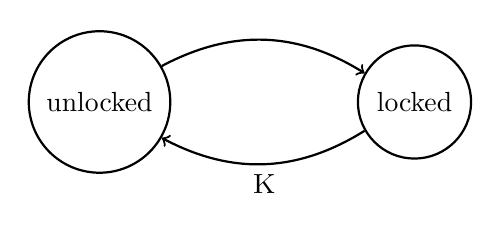
\begin{tikzpicture}[term/.style={circle,draw,thick,minimum size=8mm,inner sep=5pt},auto]
      \node (s) at (0,0) [term] {unlocked};
      \node (f) at (4,0) [term] {locked};
      \draw [->,thick] (s) to [bend left] (f);
      \draw [->,thick] (f) to [bend left] node {$\key$} (s);
    \end{tikzpicture}
  \end{center}
  The label on the transition means that the transition is only valid when we have the token $\key$, \ie{} we can only unlock a lock if we have the key.

  There are now five proof obligations, one for each of the conjuncts in the specification, and we treat each in turn.

  The first says that $\isLock(v,P,\gamma)$ is persistent, which it is
  because invariants and equality are persistent, and conjunction and
  existential quantification preserves persistency.

  The second says that $\locked(\gamma)$ \emph{is not} duplicable. This
  follows as $\key \cdot \key = \bot$ by definition of the resource algebra:
  $\ownGhost{\gamma}{\key} * \ownGhost{\gamma}{\key} \vdash
  \ownGhost{\gamma}{\key \cdot \key}$ by \ruleref{Own-op} which yields
  $\FALSE$ by \ruleref{Own-valid}. By transitivity of $\vdash$ we are
  done.

  The third is the specification of allocating a new lock, and hence needs the allocation of a lock invariant.
  We proceed to show the following triple:
  \begin{mathpar}
    \hoare{P}{\newLock ()}{v.\Exists \gamma.\isLock(v,P,\gamma)}
  \end{mathpar}
  By \ruleref{Ht-beta}, it suffices to show
  \begin{mathpar}
    \hoare{P}{\Ref(\False)}{v.\Exists \gamma.\isLock(v,P,\gamma)}
  \end{mathpar}
  We allocate new ghost state using \ruleref{Ghost-alloc}, as in Exercise~\ref{exercise:basic-properties-of-view-shift}, use the rule of consequence and then use \ruleref{Ht-exist}.
  We are left with proving
  \begin{mathpar}
    \hoare{\locked(\gamma) \ast P}{\Ref(\False)}{v.\Exists \gamma.\isLock(v,P,\gamma)}
  \end{mathpar}
  for some $\gamma$.
  \begin{exercise}
    Prove this.
    (Hint: Use the derived invariant allocation rule \ruleref{Ht-inv-alloc-post},
    and \ruleref{Ht-bind} with an empty context -).
  \end{exercise}
  
  
  The fourth is the specification of the $\acquire$ operation. It is a recursive definition, so we proceed with the derived rule for recursive functions from Exercise~\ref{exercise:derived-rule-recursive-functions}. That is, assuming 
  \begin{align}
    \All v, P, \gamma.\hoare{\later\isLock(v,P,\gamma)}{\acquire v}{\_. P \ast \locked(\gamma)}\label{eq:ih-acquire}
  \end{align}
  we show the following triple
  \begin{mathpar}
    \hoare{\isLock(v,P,\gamma)}{\If\CAS(v,\False,\True)then()\Else\acquire(v)}{\_. P \ast \locked(\gamma)}.    
  \end{mathpar}
  The $\isLock$ predicate gives us that $v$ is a location $\ell$
  governed by an invariant, which we can move into the context as follows:
  \begin{mathpar}
    \knowInv{\iota}{I(\ell,P,\gamma)}\proves
    \hoare{\TRUE}
    {\If\CAS(\ell,\False,\True)then()\Else\acquire(\ell)}
    {\_. P \ast \locked(\gamma)}
  \end{mathpar}
  We next evaluate the $\CAS$ expression with the \ruleref{Ht-bind} rule.
  As our intermediate step we proceed to show the following triple:
  \begin{mathpar}
    \knowInv{\iota}{I(\ell,P,\gamma)}\proves
    \hoare{\TRUE}
    {\CAS(\ell,\False,\True)}
    {u. (u = \True \ast  P \ast \locked(\gamma)) \lor (u = \False) }.    
  \end{mathpar}
  As $\CAS$ is atomic, we open the invariant to get at $\ell$, using
  \ruleref{Ht-inv-open}, and it suffices to show that
  \begin{mathpar}
    \knowInv{\iota}{I(\ell,P,\gamma)}\proves
    \hoareV{\later I(\ell,P,\gamma)}
    {\CAS(\ell,\False,\True)}
    {u. (\left(u = \True \ast P \ast \locked(\gamma)\right) \lor (u = \False)) \ast I(\ell,P,\gamma) }.    
  \end{mathpar}
  We proceed by cases on the invariant (using the rule \ruleref{Ht-disj}).
  In the first case we need to show
  \begin{mathpar}
    \knowInv{\iota}{I(\ell,P,\gamma)}\proves
    \hoareV{\later (\ell \pointsto \False \ast \locked{\gamma} * P)}
    {\CAS(\ell,\False,\True)}
    {u. (u = \True \ast P \ast \locked(\gamma) \lor  (u = \False)) \ast I(\ell,P,\gamma) }.
  \end{mathpar}
  By \ruleref{Ht-csq} it suffices to establish either choice of the
  disjunctions in the postcondition (there is one in the left of the
  separating conjuction, and one to the right, hidden in
  $I(\ell,P,\gamma)$).  We choose
  $u = \True \ast P \ast \locked(\gamma) * \ell\pointsto\True$ and
  by \ruleref{Ht-frame} and \ruleref{Ht-CAS-succ} we are done.
  
  In the second case, we show
  \begin{mathpar}
    \knowInv{\iota}{I(\ell,P,\gamma)}\proves
    \hoareV{\later (\ell \pointsto \True)}
    {\CAS(\ell,\False,\True)}
    {u. ((u = \True \ast P \ast \locked(\gamma) \lor
      (u = \False)) \ast I(\ell,P,\gamma) }.    
  \end{mathpar}
  Again we strengthen the post-condition, this time to
  $u = \False \ast \ell\pointsto\True$, and we are done by using the rule \ruleref{Ht-CAS-fail}.

  We are now ready to proceed with our use of \ruleref{Ht-bind}, the evaluation of the $\langkw{if}$, and the following obligation remains:
  \begin{mathpar}
    \knowInv{\iota}{I(\ell,P,\gamma)}\proves
    \hoare
    {u = \True \ast P \ast \locked(\gamma) \lor u = \False}
    {\If u then ()\Else\acquire\ell}
    {\_.P * \locked(\gamma)}
  \end{mathpar}
  We consider the two cases in the precondition, using \ruleref{Ht-disj}.
  We use \ruleref{Ht-If-True} and \ruleref{Ht-If-False} in the first and second case respectively, which leaves the following two obligations:
  \begin{align*}
    \knowInv{\iota}{I(\ell,P,\gamma)}&\proves
    \hoare
    {P \ast \locked(\gamma)}
    {()}
    {\_.P * \locked(\gamma)}\\
    \knowInv{\iota}{I(\ell,P,\gamma)}&\proves
    \hoare
    {\TRUE}
    {\acquire\ell}
    {\_.P * \locked(\gamma)}       
  \end{align*}
  The first follows by the rule for the unit expressions, the second by our induction hypothesis \eqref{eq:ih-acquire}.
  This concludes the proof that $\acquire$ satisfies its specification.
    
  The fifth and final is the specification of the $\release$ operation. We proceed to show the following triple:
  \begin{mathpar}
    \hoare{\isLock(v,P,\gamma) \ast P \ast \locked(\gamma)}{\release v}{\_.\TRUE}
  \end{mathpar}
  By definition, $\isLock(v,P,\gamma)$ tells us there is a location governed by an invariant, and we can substitute this location into the expression under evaluation, and by \ruleref{Ht-beta} we can unfold the definition of $\release$:
  \begin{mathpar}
    \hoare{\knowInv{\iota}{I(\ell,P,\gamma)} \ast P \ast \locked(\gamma)}{\ell \gets \False}{\_.\TRUE}
  \end{mathpar}
  To perform the assignment we must obtain $\ell$ as a resource from the invariant, which we do by opening it with the \ruleref{Ht-inv-open} rule. As invariants are persistent, we can move it into our assumptions before opening, leaving us with the following triple:
  \begin{mathpar}
    \knowInv{\iota}{I(\ell,P,\gamma)}\vdash
    \hoare{\later I(\ell,P,\gamma) \ast P \ast \locked(\gamma)}{\ell \gets \False}{\_.\later I(\ell,P,\gamma)}
  \end{mathpar}
  We consider two cases, based on the disjunction in $I(\ell,P,\gamma)$ in the precondition.
  The first case is
  \begin{mathpar}
    \knowInv{\iota}{I(\ell,P,\gamma)}\vdash\hoare
    {\later\left(\ell \pointsto\False \ast \locked(\gamma) \ast P\right) \ast P \ast \locked(\gamma)}{\ell \gets \False}{\_.\later I(\ell,P,\gamma)}
  \end{mathpar}
  which is inconsistent as $\locked(\gamma) \ast \locked(\gamma) \vdash \FALSE$, as argued above.
  We are done by \ruleref{Ht-later-false}.
  In the second case we need to prove
  \begin{mathpar}
    \knowInv{\iota}{I(\ell,P,\gamma)}\vdash\hoare
    {\later(\ell \pointsto\True) \ast P \ast \locked(\gamma)}{\ell \gets \False}{\_.\later I(\ell,P,\gamma)}
  \end{mathpar}
  and in the postcondition we chose the first disjunct by
  \ruleref{Ht-csq} -- \ie{} we will show the following triple:
  \begin{mathpar}
    \knowInv{\iota}{I(\ell,P,\gamma)}\vdash\hoare
    {\later(\ell \pointsto\True) \ast \later(P \ast \locked(\gamma))}{\ell \gets \False}{\_.\later (\ell \pointsto \False) \ast \later(\locked(\gamma) \ast P)}
  \end{mathpar}
  which holds by the frame rule and \ruleref{Ht-store}.
\end{example}

To show how the lock specification can be used, we use it in an example program:
We implement a concurrent bag, using the spin lock to guard access to
a shared location containing the data in the bag. 

\newcommand{\isBag}{\operatorname{isBag}}
\newcommand{\baglist}{\operatorname{bagList}}
\newcommand{\newBag}{\operatorname{newBag}}
\newcommand{\binsert}{\operatorname{insert}}
\newcommand{\bremove}{\operatorname{remove}}
\newcommand{\lock}{\operatorname{lock}}

\begin{example}[Concurrent coarse-grained bag]
  \label{example:course-grained-bag}
  The implementation is as follows.
  Recall we use syntactic sugar $\None$ for $\Inj{1} \TT$ and $\Some x$ for $\Inj{2} x$.
  The $\newBag$ method allocates a new reference cell which initially contains $\None$, together with a new lock.
  This lock is used to guard access to the location in $\binsert$ and $\bremove$ methods.
  The location will always contain a list of values.
  The $\binsert$ and $\bremove$ methods insert and remove elements.
  The $\bremove$ method returns either $\None$, in the case the bag is empty, or $\Some v$, where $v$ is the head element of the non-empty list.
  \begin{align*}
    \langkw{let} \newBag = \Lam \_ . &(\Ref(\None), \newLock \TT)\\
    \langkw{let} \binsert = \Lam x . \Lam v . &\Let \ell = \Proj{1} x in\\
                                              &\Let \lock = \Proj{2} x in\\
                                              &\acquire \lock ;\\
                                              & \ell \gets \Some (v, \deref \ell) ;\\
                                              & \release \lock\\
    \langkw{let} \bremove = \Lam x . &\Let \ell = \Proj{1} x in\\
                                     &\Let \lock = \Proj{2} x in\\
                                     &\acquire \lock ;\\
                                     &\langkw{let}\ r = \MatchML{\deref \ell}with{\None}=>{\None}|{\Some p}=>{\ell \gets \Proj{2}{p} ; \Some (\Proj{1}{p})}end{} \\
                                     & \langkw{in}\ \release \lock ; r
  \end{align*}
  We would like to have a specification of the bag which will allow
  clients to use it in a concurrent setting, where different threads insert and remove elements from a bag.

  A weak, but still useful specification is the following.  Given a
  predicate $\Phi$, the bag contains elements $x$ for which $\Phi(x)$
  holds.  When inserting an element we give away the resources, and
  when removing an element we give back an element plus the knowledge
  that it satisfies the predicate.  
  The specification is:
  \begin{align*}
    &\Exists \isBag : (\Val \to \Prop) \times \Val \to \Prop.\nonumber\\
    &\All (\Phi : \Val \to \Prop).\nonumber\\
    &\quad\quad\persistently\left(\All b . \isBag(\Phi, b) \implies \persistently \isBag(\Phi,b)\right)\\
    &\land\quad\hoare{\TRUE}{\newBag \TT}{b. \isBag(\Phi,b)}\\
    &\land\quad\All b u.\hoare{\isBag(\Phi,b) \ast \Phi(u)}{\binsert b\,u}{\_.\TRUE}\\
    &\land\quad\All b.\hoare{\isBag(\Phi,b)}{\bremove b}{v.v = \None \lor \Exists x . v = \Some x \land \Phi(x)}
  \end{align*}
  With this specification, the only thing we get to know after calling
  remove is that the returned element, if we get one out, satisfies
  the chosen predicate $\Phi$.  In fact, giving a stronger
  specification is hard.  The reason is that the $\isBag$
  predicate is freely duplicable.  And we do want the $\isBag$ to be
  duplicable, since this allows us to share it between as many threads
  as we need, which in turn allows us to specify and prove concurrent
  programs.  The consequence of $\isBag$ being duplicable is that
  concurrently running threads will be able to add and remove elements, so
  each thread has no guarantee  which particular elements it will
  get back when calling $\bremove$.
  
  We now proceed to show that the implementation meets the
  specification. The $\isBag$ predicate is defined as follows:
  \begin{align*}
    \isBag(\Phi, b) = \Exists \ell v \gamma . b = (\ell, v) \land \isLock(v, \Exists xs . \ell \pointsto xs \ast \baglist(\Phi,xs), \gamma)
  \end{align*}
  where $\baglist$ is defined by guarded recursion as the unique predicate satisfying
  \begin{align*}
    \baglist(\Phi,xs) = xs = \None \lor \Exists x . \Exists r . xs = \Some (x, r) \land \Phi(x) \ast \later(\baglist(\Phi,r)).
  \end{align*}
  Let $\Phi : \Val \to \Prop$ be arbitrary.

  \begin{exercise}
    Prove that $\isBag(\Phi,b)$ is persistent for any $b$.
  \end{exercise}
  

  \begin{exercise}
    Prove the $\newBag$ specification:
    \begin{displaymath}
      \hoare{\TRUE}{\newBag \TT}{b. \isBag(\Phi,b)}.\qedhere
    \end{displaymath}
  \end{exercise}
  

  Note that since $\isBag(\Phi,b)$ is persistent for any $b$ we can derive, by using the frame rule (exercise!), the following specification
  \begin{align*}
    \All b.\hoare{\isBag(\Phi,b)}{\bremove b}{v.\left(v = \None \lor \Exists x . v = \Some x \land \Phi(x)\right) \ast \isBag(\Phi,b)}
  \end{align*}
  from the one claimed above, \ie{} we do not lose the knowledge that $b$ is a bag.

  Let us now prove the specification of the $\bremove$ method.
  We are proving
  \begin{align*}
    \hoare{\isBag(\Phi,b)}{\bremove b}{v.v = \None \lor \Exists x . v = \Some x \land \Phi(x)}
  \end{align*}
  for some value $b$.
  
  By definition of $\isBag(\Phi,b)$ and by using \ruleref{Ht-exist}, and then \ruleref{Ht-persistently} together with \ruleref{Ht-Eq} we have to prove
  \begin{align*}
    \hoare{\isLock(\lock, \Exists xs . \ell \pointsto xs \ast \baglist(\Phi,xs), \gamma)}{\bremove (\ell,\lock)}{u.u = \None \lor{} \Exists x . u = \Some x \land \Phi(x)}
  \end{align*}
  for some $\ell$, $\lock$ and $\gamma$.
  Using \ruleref{Ht-beta} and \ruleref{Ht-let-det} we reduce to showing
  \begin{align*}
    \hoare{\isLock(\lock, \Exists xs . \ell \pointsto xs \ast \baglist(\Phi,xs), \gamma)}{e}{u.u = \None \lor{} \Exists x . u = \Some x \land \Phi(x)}
  \end{align*}
  where $e$ is the program
  \begin{align*}
    &\acquire \lock ;\\
    &\langkw{let}\ r = \MatchML{\deref \ell}with{\None}=>{\None}|{\Some p}=>{\ell \gets \Proj{2}{p} ; \Some (\Proj{1}{p})}end{} \\
    & \langkw{in}\ \release \lock ; r
  \end{align*}
  Using the sequencing rule \ruleref{Ht-seq} we use the specification of $\acquire$ as the first triple, and thus we have to prove
  \begin{align*}
    \hoare{\locked(\gamma) \ast \Exists xs . \ell \pointsto xs \ast \baglist(\Phi,xs)}{e'}{u.u = \None \lor{} \Exists x . u = \Some x \land \Phi(x)}
  \end{align*}
  where $e'$ is the part of program $e$ after $\acquire$.

  Using the fact that $\exists$ and $\lor$ distribute over $\ast$ (see Figure~\ref{fig:laws-interaction-of-connectives} on page~\pageref{fig:laws-interaction-of-connectives}), \ruleref{Ht-exist} and then the definition of $\baglist(\Phi,xs)$ together with \ruleref{Ht-disj} we consider two cases.
  The first case is
  \begin{align*}
    \hoare{\locked(\gamma) \ast \ell \pointsto xs \ast xs = \None}{e'}{u.u = \None \lor{} \Exists x. u = \Some x \land \Phi(x)}
  \end{align*}
  \begin{exercise}
    Prove the above triple (possibly after looking at the proof of the second case below).
  \end{exercise}
  

  In the second case, after using rules in Figure~\ref{fig:laws-interaction-of-connectives} and \ruleref{Ht-exist}, we get the following proof obligation.
  \begin{align*}
    \hoare{\locked(\gamma) \ast \ell \pointsto xs \ast xs = \Some(x, r) \ast \Phi(x) \ast \later \baglist(\Phi,r)}{e'}{u.u = \None \lor{} \Exists x. u = \Some x \land \Phi(x)}
  \end{align*}
  which simplifies, by \ruleref{Ht-Eq} and the rule of consequence, to proving
  \begin{align*}
    \hoare{\locked(\gamma) \ast \ell \pointsto \Some(x, r) \ast \Phi(x) \ast \later \baglist(\Phi,r)}{e'}{u.\Exists x. u = \Some x \land \Phi(x)}.
  \end{align*}
  We use the let rule \ruleref{Ht-let-det}.
  For the first premise we show
  \begin{align*}
    \hoareV{\locked(\gamma) \ast \ell \pointsto \Some(x, r) \ast \Phi(x) \ast \later \baglist(\Phi,r)}{\MatchML{\deref \ell}with{\None}=>{\None}|{\Some p}=>{\ell \gets \Proj{2}{p} ; \Some (\Proj{1}{p})}end{}}{u.u = \Some x \land \ell \pointsto r \ast \Phi(x) \ast \locked(\gamma) \ast \baglist(\Phi,r)}
  \end{align*}
  (note the omission of $\later$ on $\baglist$ in the postcondition).
  We start with the bind rule, then the \ruleref{Ht-load} rule and then \ruleref{Ht-Match} which means we have to show
  \begin{align*}
    \hoareV{\locked(\gamma) \ast \ell \pointsto \Some(x, r) \ast \Phi(x) \ast \later \baglist(\Phi,r)}{\ell \gets \pi_2(x, r) ; \Some(\pi_1 (x,r))}{u.u = \Some x \land \ell \pointsto r \ast \Phi(x) \ast \locked(\gamma) \ast \baglist(\Phi,r)}
  \end{align*}
  which by using \ruleref{Ht-bind} and \ruleref{Ht-Proj} simplifies to showing
  \begin{align*}
    \hoareV{\locked(\gamma) \ast \ell \pointsto \Some(x, r) \ast \Phi(x) \ast \later \baglist(\Phi,r)}{\ell \gets r ; \Some(\pi_1 (x,r))}{u.u = \Some x \land \ell \pointsto r \ast \Phi(x) \ast \locked(\gamma) \ast \baglist(\Phi,r)}
  \end{align*}
  Using the sequencing rule we first show
  \begin{align*}
    \hoareV{\locked(\gamma) \ast \ell \pointsto \Some(x, r) \ast \Phi(x) \ast \later \baglist(\Phi,r)}{\ell \gets r }{\_. \ell \pointsto r \ast \Phi(x) \ast \locked(\gamma) \ast \baglist(\Phi,r)}
  \end{align*}
  by using \ruleref{Ht-frame-atomic} to remove the $\later$ on $\baglist$.
  The second premise of the sequence rule, the triple
  \begin{align*}
    \hoareV{\ell \pointsto r \ast \Phi(x) \ast \locked(\gamma) \ast \baglist(\Phi,r)}
    {\Some (\pi_1(x, r))}
    {u.u = \Some x \land \ell \pointsto r \ast \Phi(x) \ast \locked(\gamma) \ast \baglist(\Phi,r)}
  \end{align*}
  is then easy to establish. Exercise!

  Finally, we need to establish the second premise of the rule \ruleref{Ht-let-det}, which means showing
  \begin{align*}
    \hoareV{\ell \pointsto r \ast \Phi(x) \ast \locked(\gamma) \ast \baglist(\Phi,r)}
    {\release \lock ; \Some x}
    {u.\Exists x. u = \Some x \land \Phi(x)}
  \end{align*}
  We can use the sequencing rule together with the $\release$ specification to give away the resources $\ell \pointsto r$, $\locked(\gamma)$ and $\baglist(\Phi,r)$ back to the lock.
  We are left with proving
  \begin{align*}
    \hoareV{\Phi(x)}
    {\Some x}
    {u.\Exists x. u = \Some x \land \Phi(x)}
  \end{align*}
  which is immediate.

  \begin{remark}
    Note that even if we did not call $\release$ we could have proved the same triple, by using weakening, \ie{} the rule $P \ast Q \proves P$.
    Such an implementation would indeed be safe, but we could never remove more than one element from the bag, since we would not be able to acquire a lock more than once.
    This is a general observation about an affine program logic such as Iris.
    However in Iris it is possible to give a stronger specification to the lock module which can ensure that locks which are acquired must be released, however this requires a more sophisticated use of the Iris base logic, so we do not dwell on it here, and instead focus only on safety specifications.
  \end{remark}
  \begin{exercise}
    Prove the specification of the $\binsert$ method:
    \begin{displaymath}
      \All b u.\hoare{\isBag(\Phi,b) \ast \Phi(u)}{\binsert b\,u}{\_.\TRUE} \qedhere
    \end{displaymath}
  \end{exercise}
  
\end{example}

\subsection{Authoritative resource algebra: counter modules}
\label{sec:authoritative-ra}

\newcommand{\isCounter}{\operatorname{isCounter}}
\newcommand{\incrC}{\operatorname{incr}}
\newcommand{\readC}{\operatorname{read}}
\newcommand{\newC}{\operatorname{newCounter}}

In this section we will endeavour to specify a counter module that can be used simultaneously by many different threads.
We will see that to achieve this we will have to introduce a new kind of resource algebra, the \emph{authoritative resource algebra}.

A first attempt at a specification is as follows.
The counter module has three methods, $\newC$ for creating a fresh counter, $\incrC$ for increasing the value of the counter, and $\readC$ for reading the current value of the counter.
There is an abstract predicate $\isCounter(v,n)$ which should state that $v$ is a counter whose current value is $n$.
This predicate should be persistent, so different threads can access the counter simultaneously.
For this reason $\isCounter(v, n)$ cannot state that $n$ is \emph{exactly} the value of the counter, but only its lower bound.
The reason we can specify the lower bound is that the counter can only increase in value.
Hence in particular other threads can only increase the value of the counter, hence they can never invalidate our lower bound.

With this, the specification of the $\incrC$ method is straightforward: the lower bound of the value of the counter is increased by $1$, and moreover the increment returns the original value of the counter, of which we know the lower bound.
\begin{align*}
  \All v . \All n . \hoare{\isCounter(v, n)}{\incrC v}{u.u \geq n \ast \isCounter(v, n+1)}.
\end{align*}
Following the discussion above, when reading the value of the counter it might be larger than that known to us via the $\isCounter$ predicate, \ie{} other threads might have increased its value without us knowing it.
\begin{align*}
  \All v . \All n . \hoare{\isCounter(v, n)}{\readC v}{u.u \geq n}
\end{align*}

The counter implementation we have in mind is the following.
The $\newC$ method creates the counter, which is simply a location containing the counter value.
\begin{align*}
  \newC \TT =\ \Ref(0)
\end{align*}
The $\incrC$ method increases the value of the counter by $1$.
Since $\ell \gets \deref \ell + 1$ is not an atomic operation we use a $\CAS$ loop, as seen in examples before.
\begin{align*}
  \Rec{\incrC} \ell =\ &\Let n = \deref \ell in\\
                       &\Let m = n + 1 in\\
                       &\If \CAS(\ell, n, m) then n \Else \incrC \ell
\end{align*}
Finally the read method simply reads the value
\begin{align*}
  \readC \ell = \deref \ell.
\end{align*}

Now, what should the $\isCounter$ predicate be?
A first attempt might be simply
\begin{align*}
  \isCounter(\ell, n) = \ell \pointsto n.
\end{align*}
However this clearly cannot work, since such an $\isCounter$ predicate is not persistent.
A second attempt might be to put the points-to assertion into the invariant as
\begin{align*}
  \isCounter(\ell, n) = \Exists \iota . \knowInv{\iota}{\ell \pointsto n}.
\end{align*}
This gets us closer, but the problem is that $\ell \pointsto n$ is not an invariant of all the methods, \ie{} not all the methods maintain this invariant.
In particular the increment method does not.
Recall that we can never change the assertion stored in the invariant, \eg{} we cannot change $\knowInv{\iota}{\ell \pointsto n}$ into $\knowInv{\iota}{\ell \pointsto (n+1)}$.
An invariant would be $\Exists m . \ell \pointsto m$, but now we need to somehow relate $m$ to $n$ which is the parameter of the $\isCounter$ predicate.
An idea might be to use the invariant
\begin{align*}
  \Exists m . \ell \pointsto m \land m \geq n
\end{align*}
and thus have
\begin{align*}
  \isCounter(\ell, n) = \Exists \iota . \knowInv{\iota}{\Exists m . \ell \pointsto m \land m \geq n}.
\end{align*}
This is an invariant, however it is not strong enough.
We cannot prove the increment method using this invariant since we cannot update $\isCounter(\ell, n)$ to $\isCounter(\ell, n+1)$, because we cannot change the assertion in the invariant.
We can conclude that any attempt which mentions $n$ in the invariant directly must fail, so we need some other way to relate the real counter value $m$ and the lower bound $n$.
We will use ghost state.
The idea is that in the invariant we will have some ghost state dependent on $m$, let us call it $\ownGhost{\gamma}{\authfull m}$, whereas we will keep some other piece of ghost state in the $\isCounter(\ell, n)$ predicate outside the invariant.
Let us call this piece $\ownGhost{\gamma}{\authfrag n}$.
Let us see what we need from the resource algebra to be able to verify the counter example by using
\begin{align}
  \label{eq:iscounter-cc-reppred}
  \isCounter(\ell, n, \gamma) = \ownGhost{\gamma}{\authfrag n} \ast \Exists \iota . \knowInv{\iota}{\Exists m . \ell \pointsto m \ast \ownGhost{\gamma}{\authfull m}}
\end{align}
as the abstract predicate.
First, to verify the read method we will open the invariant, and after some simplification we will have $\ownGhost{\gamma}{\authfull m \cdot \authfrag n}$ and the value we are going to return is $m$.
From this we should be able to conclude that $m \geq n$.
Using \ruleref{Own-valid} we have $\authfull m \cdot \authfrag n \in \Vl$, where $\Vl$ is the set of valid elements of the resource algebra we are trying to define.
Hence we need to be able to conclude $m \geq n$ from $\authfull m \cdot \authfrag n \in \Vl$.
Next, if $\isCounter(\ell, n, \gamma)$ is to be persistent, it must be that $\ownGhost{\gamma}{\authfrag n}$ is persistent, which is only the case (see \ruleref{Persistently-core}) if $\mcore{\authfrag n} = \authfrag{n}$, where $\mcore{\cdot}$ is the core operation of the resource algebra we are defining.
In particular this means that $\authfrag n$ must be duplicable for any $n$.

Finally, let us see what we need to verify the $\incrC$ method.
As we have seen many times by now, we have to update the ghost state when the $\CAS$ operation succeeds.
Just before the $\CAS$ operation succeeds the following resources are available
\begin{align*}
  \ell \pointsto k \ast \ownGhost{\gamma}{\authfull k \cdot \authfrag n}
\end{align*}
and just after we will have
\begin{align*}
  \ell \pointsto (k+1) \ast \ownGhost{\gamma}{\authfull k \cdot \authfrag n}.
\end{align*}
Using these we need to reestablish the invariant, and get $\ownGhost{\gamma}{\authfrag (n+1)}$ in order to conclude
\begin{align*}
  \isCounter(\ell, n+1, \gamma).
\end{align*}
The only way to do this is to update the ghost state using \ruleref{Ghost-update}.
Thus it would suffice to have the frame preserving update
\begin{align*}
  \authfull k \cdot \authfrag n \mupd \authfull (k+1) \cdot \authfrag (n+1).
\end{align*}

To recap, here are the requirements of our resource algebra.
\begin{align}
  \label{eq:1:core-of-auth-max}
  &\mcore{\authfrag n} = \authfrag{n}\\
  \label{eq:2:valid-of-auth-max}
  &\authfull m \cdot \authfrag n \in \Vl \implies m \geq n\\
  \label{eq:3:valid-update-auth-max}
  &\authfull m \cdot \authfrag n \mupd \authfull (m+1) \cdot \authfrag (n+1)
\end{align}
We now define a resource algebra which allows us to achieve these properties.
Let $\Ml = \NN_{\bot,\top} \times \NN$ where $\NN_{\bot,\top}$ is the set of natural numbers with two additional elements $\bot$ and $\top$.
Define the operation $\cdot$ as
\begin{align*}
  (x, n) \cdot (y, m) =
  \begin{cases}
    (y, \max(n, m)) & \text{ if } x = \bot\\
    (x, \max(n, m)) & \text{ if } y = \bot\\
    (\top, \max(n, m)) & \text{ otherwise}
  \end{cases}
\end{align*}
It is easy to see (exercise!) that this makes $\Ml$ into a commutative semigroup.
Moreover it has a unit, which is the element $(\bot, 0)$.

For $m, n \in \NN$ let us write $\authfull m$ for $(m, 0)$ and $\authfrag n$ for $(\bot, n)$.
Using the definition of the operation we clearly see $\authfull m \cdot \authfrag n = (m, n)$.
Thus to get property~\eqref{eq:2:valid-of-auth-max} we should require that if $(m, n) \in \Vl$ for natural numbers $n$ and $m$ then $m \geq n$.
Moreover, the closure condition of the set of valid elements states that subparts of valid elements must also be valid.
Thus, since we wish $(n, n) = \authfrag n \cdot \authfull n \in \Vl$ we must also have $\authfrag n = (\bot, n) \in \Vl$.
With this in mind we define the set of valid elements as
\begin{align*}
  \Vl = \left\{(x, n) \isetsep x = \bot \lor x \in \NN \land x \geq n\right\}.
\end{align*}
In particular note that elements of the form $(\top, n)$ are \emph{not} valid.
With this definition we can see that property~\eqref{eq:2:valid-of-auth-max} holds.

Requirement~\eqref{eq:1:core-of-auth-max} defines the core on elements $\authfrag n$.
The only way to extend it to the whole $\Ml$ so that it still satisfies all the axioms of the core is to define
\begin{align*}
  \mcore{(x, n)} = (\bot, n).
\end{align*}
It is easy to see that this definition makes $(\Ml, \Vl, \mcore{\cdot})$ into a unital resource algebra.

Finally, let us check we have property~\eqref{eq:3:valid-update-auth-max}.
Recall Definition~\ref{def:frame-preserving-update} (on page~\pageref{def:frame-preserving-update}) of frame preserving updates.
Let $(x, y) \in \Ml$ be such that $(\authfull m \cdot \authfrag n) \cdot (x, y)$ is valid.
This means in particular that $x = \bot$ and that $m \geq \max(n, y)$.
Hence $m+1 \geq \max(n+1,y)$ and thus $(\authfull (m+1) \cdot \authfrag (n+1)) \cdot (x, y)$ is also valid, as needed.

In particular note how it was necessary that $\authfull m \cdot \authfull k = (\top, 0)$ is \emph{not} valid to conclude that $x$ must be $\bot$, which is why we define the operation in this rather peculiar way.

\begin{exercise}
  \label{exercise:simple-counter-specification}
  Let $\isCounter : \Val \to \NN \to \textlog{GhostName} \to \Prop$ be the predicate
  \begin{align*}
    \isCounter(\ell, n, \gamma) = \ownGhost{\gamma}{\authfrag n} \ast \Exists \iota . \knowInv{\iota}{\Exists m . \ell \pointsto m \ast \ownGhost{\gamma}{\authfull m}}.
  \end{align*}
  Show the following specifications for the methods defined above.
  \begin{align*}
    &\hoare{\TRUE}{\newC \TT}{u.\Exists \gamma . \isCounter(u, 0, \gamma)}\\
    &\All \gamma . \All v . \All n . \hoare{\isCounter(v, n, \gamma)}{\readC v}{u.u \geq n}\\
    &\All \gamma . \All v . \All n . \hoare{\isCounter(v, n, \gamma)}{\incrC v}{u.u \geq n \ast \isCounter(v, n+1,\gamma)} \tag*{\qedhere}
  \end{align*}
\end{exercise}


\begin{exercise}
  \label{exercise:simple-counter-spec-example-program}
  Let $e$ be the program
  \begin{align*}
    \Let c = \newC \TT in (\incrC c || \incrC c); \readC c.
  \end{align*}
  Using the specification of the counter module from the preceding exercise show the following specification for $e$.
  \begin{displaymath}
    \hoare{\TRUE}{e}{v.v \geq 1}. \qedhere
  \end{displaymath}
\end{exercise}


\subsubsection*{A more precise counter specification}

The specification of the program $e$ from the above exercise is the strongest possible given the specification of the counter from Exercise~\ref{exercise:simple-counter-specification}.
However operationally we know that the result of that program is exactly the value $2$.
With the $\isCounter$ predicate as above we cannot prove such a precise result simply because $\isCounter$ is freely duplicable, and so in each thread we do not know whether there are other threads using the counter, and thus possibly increasing its value.

In order to give a more precise specification to the counter we must keep track of whether we are the only ones who currently has access to the counter, or if there are possibly other threads using it.
This can be achieved by using fractions in the following way.
The $\isCounter$ will be parametrized by $q$ which indicates the degree of ownership of the counter.
If we own the full counter, \ie{} $q = 1$ then we know its exact value.
If we own only a part of it then we only know its lower bound.
The $\readC$ method thus has two specifications.
\begin{align*}
  &\All \gamma . \All v . \All n . \hoare{\isCounter(v, n, \gamma, {\color{red} 1})}{\readC v}{u.u = n}\\
  &\All q . \All \gamma . \All v . \All n . \hoare{\isCounter(v, n, \gamma, {\color{red} q})}{\readC v}{u.u \geq n}
\end{align*}
The increment has an analogous specification, apart from it being parametrized by $q$, and the $\newC$ method creates a counter which is owned in full by the thread that created it.

The next question is how do we share the counter.
As explained above, the $\isCounter$ predicate cannot be persistent.
Instead, when splitting the counter we must record that somebody else can also use it.
We achieve this by parameterising the counter predicate with an additional fraction $p \in (0, 1]$.
This fraction indicates our degree of knowledge about the counter.
If $p=1$ we have the full ownership of the counter, and thus can know its exact value.
Otherwise we only know its lower bound as with the previous counter specification.
By using the following splitting property of the new $\isCounter$ predicate
\begin{align*}
  \isCounter(v, n, \gamma, p) \ast \isCounter(v, m, \gamma, q) \provesIff \isCounter(v, n + m, \gamma, p + q)
\end{align*}
we can create the counter, share it among different threads, and then once all of those threads are finished executing we can combine all the counters and read off the exact value.

In light of this rule there is another way to read the assertion $\isCounter(v, n, \gamma, p)$.
We can read it as that the contribution of this thread to the total value of the counter is exactly $n$.
If $p$ is $1$ then this is the only thread, and so the value of the counter is exactly $n$.

To define the desired $\isCounter$ predicate and to prove the desired specification we will need a resource algebra similar to the one used for the first counter specification, but more involved.
To achieve it we need to generalize the resource algebra we have defined above to the construction called \emph{authoritative resource algebra}.

\begin{example}[Authoritative resource algebra]
  \label{example:authoritative-RA}
  Given a \emph{unital} resource algebra $\Ml$ with unit $\eps$, set of valid elements $\Vl$ and core $\mcore{\cdot}$, let $\authm(\Ml)$ be the resource algebra whose carrier is the set $\Ml_{\bot,\top} \times \Ml$ (recall that $\Ml_{\bot,\top}$ is the set $\Ml$ together with two new elements $\bot$ and $\top$) and whose operation is defined as
  \begin{align*}
    (x, a) \cdot (y, b) =
    \begin{cases}
      (y, a \cdot b) & \text{ if } x = \bot\\
      (x, a \cdot b) & \text{ if } y = \bot\\
      (\top, a \cdot b) & \text{ otherwise }
    \end{cases}
  \end{align*}
  The core function is defined as (recall that the core is total in a unital resource algebra; see Exercise~\ref{exercise:unital-ra-core-total})
  \begin{align*}
    \mcore{(x, a)}_{\authm(\Ml)} = \left(\bot, \mcore{a}\right)
  \end{align*}
  and the set of valid elements is
  \begin{align*}
    \Vl_{\authm(\Ml)} = \left\{(x, a) \isetsep x = \bot \land a \in \Vl \lor x \in \Ml \land x \in \Vl \land  a \mincl x\right\}
  \end{align*}
  We write $\authfull m$ for $(m,\eps)$ and $\authfrag n$ for $(\bot,n)$.
\end{example}
\begin{exercise}
  Show that the resource algebra $\Ml$ we used in the counter specification in Exercise~\ref{exercise:simple-counter-specification} is exactly the resource algebra $\authm(\NN_{\max{}})$ where $\NN_{\max{}}$ is the resource algebra whose carrier is the set of natural numbers, and its operation the maximum.
  Its core is the identity function and all elements are valid.
\end{exercise}


\begin{exercise}
  Show the following properties of the resource algebra $\authm(\Ml)$ for an arbitrary \emph{unital} resource algebra $\Ml$.
  \begin{itemize}
  \item $\authm(\Ml)$ is unital with unit $(\bot, \eps)$, where $\eps$ is the unit of $\Ml$
  \item $\authfull x \cdot \authfull y \notin \Vl_{\authm(\Ml)}$ for any $x$ and $y$
  \item $\authfrag x \cdot \authfrag y = \authfrag (x \cdot y)$
  \item $\authfull x \cdot \authfrag y \in \Vl \implies y \mincl x$
  \item if $x \cdot z$ is valid in $\Ml$ then
    \begin{align*}
      \authfull x \cdot \authfrag y \mupd \authfull (x \cdot z) \cdot \authfrag (y \cdot z)
    \end{align*}
    in $\authm(\Ml)$.
  \item if $x \cdot z$ is valid in $\Ml$ and $w \mincl z$ then
    \begin{align*}
      \authfull x \cdot \authfrag y \mupd \authfull (x \cdot z) \cdot \authfrag (y \cdot w)
    \end{align*}
    in $\authm(\Ml)$.
  \end{itemize}
\end{exercise}


Recall the $\isCounter$ predicate we used previously
\begin{align*}
  \isCounter(\ell, n, \gamma) = \ownGhost{\gamma}{\authfrag n} \ast \Exists \iota . \knowInv{\iota}{\Exists m . \ell \pointsto m \ast \ownGhost{\gamma}{\authfull m}}.
\end{align*}
We wish to incorporate into it the fraction $p$ indicating how much of the counter this thread owns.
We do this as follows.
\begin{align*}
  \isCounter(\ell, n, \gamma, p) = \ownGhost{\gamma}{\authfrag (p, n)} \ast \Exists \iota . \knowInv{\iota}{\Exists m . \ell \pointsto m \ast \ownGhost{\gamma}{\authfull (1, m)}}.
\end{align*}
Thus the invariant stores the exact value of the counter, and since it knows its exact value the fraction is $1$.
The assertion $\ownGhost{\gamma}{\authfrag (p, n)}$ connects the actual value of the counter to the value that is known to the particular thread.
Now, to be able to read the exact value of the counter when $p$ is $1$ we need the property that if $\authfull (1, m) \cdot \authfrag (1, n)$ is valid then $n = m$.
Further, we need the property that if $\authfull (1, m) \cdot \authfrag (p, n)$ is valid then $m \geq n$.
Finally, we wish to get $\isCounter(\ell, n + k, \gamma, p + q) \provesIff \isCounter(\ell, n, \gamma, p) \ast \isCounter(\ell, k, \gamma, q)$.
The way to achieve all this is to take the resource algebra $\authm\left(\left(\QQ_{01} \times \NN\right)_?\right)$ where
\begin{itemize}
\item $\QQ_{01}$ is the resource algebra of fractions from Example~\ref{example:resource-algebra-of-fractions},
\item $\NN$ is the resource algebra of natural numbers with \emph{addition} as the operation, and every element is valid,
\item and $\left(\QQ_{01} \times \NN\right)_?$ is the option resource algebra on the product of the two previous ones.
\end{itemize}

\begin{exercise}
  \label{exercise:properties-of-fractional-natural-auth-ra}
  Show the following properties of the resource algebra $\left(\QQ_{01} \times \NN\right)_?$.
  \begin{itemize}
  \item $(p, n) \cdot (q, m) = (p + q, n + m)$
  \item if $q \leq 1$ then $(p, n) \mincl (q, m)$ if and only if
    \begin{itemize}
    \item $p \leq q$ and $n \leq m$ (where $\leq$ is the standard ordering on naturals and rationals)
    \item if $p = 1$ then $q = 1$ and $n = m$.
    \end{itemize}
  \end{itemize}
  And show the following properties of the resource algebra $\authm\left(\left(\QQ_{01} \times \NN\right)_?\right)$.
  \begin{itemize}
  \item $\authfrag (p, n) \cdot \authfrag (q, m) = \authfrag(p + q, n + m)$
  \item if $\authfull (1, m) \cdot \authfrag(p, n)$ is valid then $n \leq m$ and $p \leq 1$
  \item if $\authfull (1, m) \cdot \authfrag(1, n)$ is valid then $n = m$
  \item $\authfull (1, m) \cdot \authfrag (p, n) \mupd \authfull (1, m+1) \cdot \authfrag (p, n+1)$.\qedhere
  \end{itemize}
\end{exercise}

Using the results from the preceding exercise about ghost updates the following exercise is a straightforward adaptation of Exercise~\ref{exercise:simple-counter-specification}.
\begin{exercise}
  \label{exercise:precise-counter-specification}
  Let $\isCounter$ be the predicate
  \begin{align*}
    \isCounter(\ell, n, \gamma, p) = \ownGhost{\gamma}{\authfrag (p, n)} \ast \Exists \iota . \knowInv{\iota}{\Exists m . \ell \pointsto m \ast \ownGhost{\gamma}{\authfull (1, m)}}.
  \end{align*}
  First show that for any $p, q, n$, and $k$, we have
  \begin{align*}
    \isCounter(\ell, n + k, \gamma, p + q) \provesIff \isCounter(\ell, n, \gamma, p) \ast \isCounter(\ell, k, \gamma, q).
  \end{align*}

  Next show the following specifications for the methods defined above.
  \begin{align*}
    &\hoare{\TRUE}{\newC \TT}{u.\Exists \gamma . \isCounter(u, 0, \gamma, 1)}\\
    &\All p . \All \gamma . \All v . \All n . \hoare{\isCounter(v, n, \gamma, p)}{\readC v}{u.u \geq n}\\
    &\All \gamma . \All v . \All n . \hoare{\isCounter(v, n, \gamma, 1)}{\readC v}{u.u = n}\\
    &\All p . \All \gamma . \All v . \All n . \hoare{\isCounter(v, n, \gamma, p)}{\incrC v}{u.u \geq n \ast \isCounter(v, n+1,\gamma, p)} \tag*{\qedhere}
  \end{align*}
\end{exercise}

Using the specification from the previous exercise we can now revisit Exercise~\ref{exercise:simple-counter-spec-example-program} to give it the most precise specification.
\begin{exercise}
\label{exercise:precise-counter-spec-example-program}
  Let $e$ be the program
  \begin{align*}
    \Let c = \newC \TT in (\incrC c || \incrC c); \readC c.
  \end{align*}
  Using the specification of the counter module from the preceding exercise show the following specification for $e$.
  \begin{displaymath}
    \hoare{\TRUE}{e}{v.v = 2}.\qedhere
  \end{displaymath}
\end{exercise}


\subsection{Parallel composition via \texorpdfstring{$\Fork{}$}{Fork()}}
\label{sec:parcomp-from-fork}

We can now show how to derive the proof rule \ruleref{Ht-par} which we simply stated on page~\pageref{Ht-par} from the following rule for the primitive $\Fork{}$.
The primitive $\Fork{}$ rule is as follows.
\begin{mathpar}
  \inferH{Ht-fork}
  {S \proves \hoare{P}{e}{\_.\TRUE}[\mask]}
  {S \proves \hoare{P}{\Fork{e}}{v.v = \TT}[\mask]}
\end{mathpar}
The key point is that we only require the forked-off thread to be safe, we do not care about its return value, hence the post-condition $\TRUE$ in the premise.

Recall how parallel composition is defined in Section~\ref{sec:par-construct}.
It uses two auxiliary methods $\langkw{spawn}$, which creates a new thread and a ``shared channel'' which is used to signal when it is done, and the $\langkw{join}$ method which listens on the channel until the spawned thread is done.
These methods are of independent interest since, in contrast to the plain $\Fork{}$, they allow us to wait for a forked-off thread to finish.
Since we are using a shared channel we will use an invariant to allow the two threads to access it.

The method $\langkw{spawn}$ has a function $f$ as an argument.
Let us assume that $f$ has the following specification for some predicates $P$ and $v.Q$.
\begin{align*}
  \hoare{P}{f\,\TT}{v.Q}.
\end{align*}

With these parameters fixed we define the following predicate
\newcommand{\joinH}{\operatorname{joinHandle}}
\begin{align*}
  \joinH(\ell, \gamma, v.Q) \eqdef \ownGhost{\gamma}{\TT} \ast \knowInv{\iota}{\ell \pointsto \None \lor \Exists x . \ell \pointsto \Some x \ast Q(x) \lor \ell \pointsto - \ast \ownGhost{\gamma}{\TT}}.
\end{align*}
where we are using the exclusive resource algebra over the singleton set (see Example~\ref{ex:exclusive-resource-algebra}).
The idea is that the $\langkw{spawn}$ method returns this handle, which has information about the state of the forked-off thread.
In the beginning the invariant is in the first state, with the location $\ell$ pointing to $\None$.
Once the $\langkw{spawn}$ terminates the invariant will intuitively be in the second state, with $\ell \pointsto \Some x$ and $Q(x)$.

When the $\langkw{join}$ method is waiting for the location to become $\Some x$ it will have the $\ownGhost{\gamma}{\TT}$ token, allowing it to know that the invariant is either in the first or the second state.
Once it is in the second the $\langkw{join}$ method will close the invariant in the third state, transferring $\ownGhost{\gamma}{\TT}$ into it, and obtaining $Q(x)$.

\begin{exercise}
  Following the description above show the following specifications for the $\langkw{spawn}$ and $\langkw{join}$ methods in detail.
  \begin{mathpar}
    \inferH{Ht-spawn}
    {\hoare{P}{f\,\TT}{v.Q}}
    {\hoare{P}{\langkw{spawn}(f)}{\ell.\Exists \gamma . \joinH(\ell, \gamma, v.Q)}}
    \and
    \inferH{Ht-join}
    { }
    {\hoare{\joinH(\ell, \gamma, v.Q)}{\langkw{join}(\ell)}{v.Q}}
  \end{mathpar}
  Using these specifications derive the \ruleref{Ht-par} specification of the parallel composition operation.
\end{exercise}


%%% Local Variables:
%%% mode: latex
%%% TeX-master: "../main.tex"
%%% End:
